%%	SECCION documentclass																									 %%	
%%---------------------------------------------------------------------------%%
\documentclass{article}

%%---------------------------------------------------------------------------%%
%%	SECCION usepackage																											 %%	
%%---------------------------------------------------------------------------%%
\usepackage{amsmath, amsthm}
\usepackage[spanish,activeacute]{babel}
\usepackage{caratula}
\usepackage{a4wide}
\usepackage{hyperref}
\usepackage{fancyhdr}
% \usepackage{moreverb}
\usepackage{graphicx} % Para el logo magico!
\usepackage{capt-of}
\usepackage{afterpage}
\usepackage{float}
\usepackage{amssymb}
\usepackage{amsmath}
\usepackage[latin1]{inputenc}
\usepackage{subfigure}
\usepackage{algorithm}
\usepackage{algorithmic}
\usepackage[dvipsnames,usenames]{color}
\usepackage{amsfonts}
\usepackage{code_color}
\usepackage{amsthm}
\usepackage{marvosym}
%\usepackage{minipage}

%%---------------------------------------------------------------------------%%
%%	SECCION opciones																												 %%	
%%---------------------------------------------------------------------------%%
\parskip    = 11 pt
\headheight	= 13.1pt
\pagestyle	{fancy}
\definecolor{orange}{rgb}{1,0.5,0}

\addtolength{\headwidth}{1.0in}

\addtolength{\oddsidemargin}{-0.5in}
\addtolength{\textwidth}{1.0in}
\addtolength{\topmargin}{-0.8in}
\addtolength{\textheight}{0.7in}

%%%---------------------------------------------------------------------------%%
%%%	SECCION listings    													 %%	
%%%---------------------------------------------------------------------------%%
%\usepackage{listings}
%\lstset{
%		language=C++,
%		basicstyle=\ttfamily \small,
%		keepspaces=true,
%		flexiblecolumns=false,
%		basewidth={0.5em,0.45em},
%		keywordstyle=\ttfamily \bfseries \hlkwa,
%		tabsize=4
%}

%%---------------------------------------------------------------------------%%
%%	SECCION document	 %%	
%%---------------------------------------------------------------------------%%
\begin{document}
\renewcommand{\chaptername}{Parte }
\renewcommand{\algorithmicrequire}{\textcolor{blue}{\textbf{Requiere:}}}
\renewcommand{\algorithmicensure}{\textbf{Devuelve:}}
\renewcommand{\algorithmicend}{\textbf{Fin}}
\renewcommand{\algorithmicif}{\textcolor{blue}{\textbf{Si}}}
\renewcommand{\algorithmicthen}{\textcolor{blue}{}} %%\textbf{entonces}}}
\renewcommand{\algorithmicelse}{\textcolor{red}{\textbf{Si no}}}
\renewcommand{\algorithmicelsif }{\textcolor{blue}{\textbf{Si no y}}}
\renewcommand{\algorithmicendif}{\textcolor{blue}{\textbf{Fin si}}}
\renewcommand{\algorithmicfor}{\textcolor{ForestGreen}{\textbf{Para}}}
\renewcommand{\algorithmicendfor}{\textcolor{ForestGreen}{\textbf{Fin para}}}
\renewcommand{\algorithmicwhile}{\textcolor{ForestGreen}{\textbf{Mientras}}}
\renewcommand{\algorithmicendwhile}{\textcolor{ForestGreen}{\textbf{Fin mientras}}}
\renewcommand{\algorithmicdo}{\textcolor{ForestGreen}{}} %%\textbf{hacer}}}
\renewcommand{\algorithmicreturn}{\textbf{Devolver}}
\floatname{algorithm}{Algoritmo}

%%---- Caratula -------------------------------------------------------------%%
\materia{Problemas, algoritmos y programaci�n (2010)}
\titulo{Trabajo Pr'actico n� 3}


\integrante{Barenbaum, Pablo}{124/04}{foones@gmail.com}
\integrante{Mart'inez, Federico}{17/06}{federicoemartinez@gmail.com}
\integrante{Sainz-Tr'apaga, Gonzalo}{454/06}{gonzalo@sainztrapaga.com.ar}
\grupo{Grupo 1}
\resumen{
El siguiente informe presenta la resoluci�n a los 4 problemas correspondientes al tercer trabajo pr\'actico de la materia problemas, algoritmos y programaci�n en el primer cuatrimestre del 2010. En el mismo se encuentra la explicaci�n del algoritmo utilizado para resolver cada problema, as� como tambi�n la implementaci�n en C++ de los mismos.
}

% TOC, usa estilos locos
\maketitle
\pagestyle{empty}
{
\fancypagestyle{plain}
    {
    \fancyhead{}
    \fancyfoot{}
    \renewcommand{\headrulewidth}{0.0pt}
    } % clear header and footer of plain page because of ToC
%\tableofcontents
}

\newpage
% arreglos los estilos para el resto del documento, y
% reseteo los numeros de pagina para que queden bien
\pagenumbering{arabic}
\fancypagestyle{plain} {
    \fancyhead[LO]{Barenbaum, Mart�nez, Sainz Tr�paga}
    \fancyhead[C]{}
    \fancyhead[RO]{P\'agina \thepage\ de \pageref{LastPage}}
    \fancyfoot{}
    \renewcommand{\headrulewidth}{0.4pt}
}
\pagestyle{plain}
\section{11235 - Frequent values}
\textbf{Problema:} Dado un arreglo de n�meros ordenados de forma no decreciente, y un par de indices $i$, $j$; encontrar la mayor frecuencia (repeticiones de un numero) en el rango $[i,j]$ del arreglo.

\subsection{Resoluci�n}
Dado que el arreglo esta ordenado, las apariciones de un n�mero est�n todas juntas. En otras palabras, si $k$ est� en el arreglo, vale que:

$\exists i,j / k \notin a[0..i-1]  \wedge \forall t \in a[i..j], a[t] = k \wedge k \notin a[j+1..n]$

Esto es �til porque significa que todas las apariciones de un elemento est�n juntas, 
es decir que en el arreglo los elementos iguales est�n en subarreglos. Podemos 
considerar entonces el arreglo que se obtiene de considerar las longitudes de esos 
subarreglos (consideramos subarreglos m�ximos - los que abarcan todas las apariciones 
de un elemento). Por ejemplo, si el arreglo original es:
$$a = -1, -1, 1, 1, 1, 1, 3, 10, 10, 10$$
el arreglo de las cantidades es:
$$c = 2, 4, 1, 3$$

Definimos adem�s:

$s(i) = k  \longleftrightarrow c[k]$ representa al subarreglo que contiene a los elementos que son iguales a $a[i]$

$d(i) = 0 \longleftrightarrow \forall 0 \leq t \leq i, a[t] = a[i] $

$d(i) = k > 0 \longleftrightarrow a[k] = a[i] \wedge a[k-1] < a[i]$


$h(i) = n - 1  \longleftrightarrow \forall i \leq t < n, a[t] = a[i] $

$h(i) = k < n -1 \longleftrightarrow a[k] = a[i] \wedge a[k+1] > a[i]$

Intuitivamente, $d(i)$ y $h(i)$ son los extremos del intervalo en a, tal que $\forall d(i) \leq t \leq h(i), a[t] == a[i]$. Notemos entonces que vale que:

$\forall i,j / s(i) = s(j) \Rightarrow d(i)=d(j) \wedge h(i)=h(j)$

Esto es as� ya que si $s(i) = s(j)$, se desprende que $a[i] = a[j]$

El arreglo $c$ es �til para resolver el problema. Si tenemos que dar la m�xima frecuencia 
en $[i,j]$, puede pasar que:
\begin{itemize}
\item $a[i] = a[j]$, con lo cual la m�xima frecuencia es el largo de  $[i,j]$
\item $a[i] \neq a[j]$, en este caso podemos usar el arreglo $c$ para hacer una consulta 
por el m�ximo en el intervalo $[s(i)..s(j)]$. Esto s�lo es cierto si $i$ es el extremo 
izquierdo de un subarreglo de $a$, y $j$ es el extremo derecho de otro. 

Si esto no se cumple, hay que considerar que del subarreglo que corresponde 
a $i$ o a $j$ s�lo importa una parte. 

Entonces, la m�xima frecuencia se puede obtener como: 
$$max(\Vert [i..h(i)] \Vert, \Vert [d(j)..j] \Vert, max(c[s(i)+1...s(j)-1]))$$

Esto corresponde al m�ximo entre la cantidad de valores iguales a $a[i]$ que caen en el 
intervalo pedido, la cantidad de valores iguales a $a[j]$ y la m�xima frecuencia entre ellos.
\end{itemize}

Al cargar el arreglo se pueden computar $s$, $d$, $h$ y $c$, de la siguiente manera:

\begin{algorithm}[H]
\begin{algorithmic}
\caption{Calculo de $s$, $d$, $h$ y $c$ a partir del arreglo ordenado}
\PARAMS{arreglo $a$, ordenado de forma no decreciente}
\STATE $i = 0$
\STATE $actual = a[i]$
\STATE $intervalo = 0$
\STATE $desde = 0$
\STATE $hasta = 0$
\STATE $s(i) = intervalo$
\STATE $c[intervalo] = 1$
\STATE $i = 1$
\WHILE{$i < \Vert a \Vert - 1 $}
	\IF{$actual = a[i-1]$}
		\STATE $hasta++$
		\STATE $c[intervalo]++$
	\ELSE
		\STATE $h(intervalo) = hasta$
		\STATE $d(intervalo) = desde$
		\STATE $intervalo++$
		\STATE $hasta++$
		\STATE $desde = hasta$
		\STATE $actual = a[i]$
		\STATE $c[intervalo] = 1$
	\ENDIF
	\STATE $s(i) = intervalo$
	\STATE $i++$
\ENDWHILE
\STATE $h(intervalo) = hasta$
\STATE $d(intervalo) = desde$
\end{algorithmic}
\end{algorithm}

Para guardar $s,d$ y $h$ se pueden usar arreglos, e indexar $h y d$ siempre por $s(i)$.

Una vez que tenemos esto, queda computar eficientemente el m�ximo en  $c[s(i)+1...s(j)-1]$. 
Para ello usamos la estructura \textit{\textbf{Sparse Table} }\footnote{http://www.topcoder.com/tc?module=Static\&d1=tutorials\&d2=lowestCommonAncestor}.

Una vez construida esta estructura podemos comenzar a responder las consultas. El siguiente es el algoritmo para responderlas:

\begin{algorithm}[H]
\begin{algorithmic}
\caption{Resoluci�n de queries}
\PARAMS{$i,j$ indices del arreglo $a$}
\IF{s(i) == s(j)}
	\RETURN $j-i+1$ \COMMENT{$\Vert[i..j]\Vert$}
\ELSE
	\STATE res = $max( h(s(i)) - i +1, j - d(s(j)) + 1)$ \COMMENT{$max(\Vert [i..h(i)] \Vert, \Vert [d(j)..j] \Vert)$}
	\STATE res = $max(res, rmq(c, h(s(i))+1, d(s(j))-1))$ \COMMENT{usar la sparse table para obtener el maximo en el rango de c}
	\RETURN res
\ENDIF
\end{algorithmic}
\end{algorithm}

Con respecto a la complejidad, primero computamos $s,d,h$ y $c$, lo que podemos hacer en $O(n)$ mientras 
cargamos los n�meros. Luego armamos la \textit{sparse table} para el arreglo $c$, que tiene $O(n)$ elementos 
(pueden ser $n$, si todos los elementos de $a$ son distintos). Por lo tanto, la construcci�n de la tabla es 
$O(n \log n)$. Usando el algoritmo antes mostrado, podemos responder a las consultas en $O(1)$, ya que la 
consulta a la tabla cuesta $O(1)$. Por lo tanto, si hay $q$ queries que responder, el orden total del algoritmo 
es $O(n \log n + q)$. Ajustando un poco el calculo, vemos que la tabla no tiene siempre $O(n*\log n)$ posiciones, 
sino que tiene $O(d*\log d)$ posiciones, donde $d$ es la cantidad de elementos distintos. Si bien $O(d*\log d) 
\subseteq O(n*\log n)$, potencialmente $d$ es m�s chico que $n$. Considerando que igualmente deben cargarse 
todos los valores del arreglo original, el orden es $O(n + d*\log d + q)$.

\subsection{Implementaci�n}
\noindent
\ttfamily
\shorthandoff{"}\\
\hlstd{}\hlline{\ 1\ }\hldir{\#include\ $<$iostream$>$}\\
\hlline{\ 2\ }\hlstd{}\hldir{\#include\ $<$vector$>$}\\
\hlline{\ 3\ }\hlstd{}\hldir{\#include\ $<$list$>$}\\
\hlline{\ 4\ }\hlstd{}\hldir{\#include\ $<$stdlib.h$>$}\\
\hlline{\ 5\ }\hlstd{}\hldir{\#include\ $<$utility$>$}\\
\hlline{\ 6\ }\hlstd{}\hldir{\#include\ $<$cassert$>$}\\
\hlline{\ 7\ }\hlstd{}\hldir{\#include\ $<$sys/types.h$>$}\\
\hlline{\ 8\ }\hlstd{}\hldir{\#include\ $<$sys/stat.h$>$}\\
\hlline{\ 9\ }\hlstd{}\hldir{\#include\ $<$fcntl.h$>$}\\
\hlline{10\ }\hlstd{}\hldir{\#include\ $<$stdio.h$>$}\\
\hlline{11\ }\hlstd{}\hlkwa{using\ namespace\ }\hlstd{std}\hlsym{;}\\
\hlline{12\ }\hlstd{}\hldir{\#define\ forit(it,l)\ for(it=(l).begin();it\ !=\ (l).end();\ it++)}\\
\hlline{13\ }\hlstd{}\hldir{\#define\ forn(i,n)\ for(unsigned}\hlstd{\ \ }\hldir{i=\ 0;\ i\ $<$\ ((unsigned)(n));\ i++)}\\
\hlline{14\ }\hlstd{}\hldir{\#define\ foreachin(it,s)\ for(typeof((s).begin())\ it\ =\ ((s).begin());\ it\ !=\ ((s).end());\ it++)}\\
\hlline{15\ }\hlstd{}\hldir{\#define\ forsn(i,s,n)\ for(int\ i\ =\ (s);\ i\ $<$\ (n);\ i++)}\\
\hlline{16\ }\hlstd{}\hlkwb{void\ }\hlstd{}\hlkwc{inline\ }\hlstd{}\hlkwd{llenar\textunderscore tabla}\hlstd{}\hlsym{(}\hlstd{vector}\hlsym{$<$}\hlstd{vector}\hlsym{$<$}\hlstd{}\hlkwb{int}\hlstd{}\hlsym{$>$\ $>$\&\ }\hlstd{tabla}\hlsym{,\ }\hlstd{}\hlkwb{const\ }\hlstd{vector}\hlsym{$<$}\hlstd{}\hlkwb{int}\hlstd{}\hlsym{$>$\&\ }\hlstd{frec}\hlsym{)\ \{}\\
\hlline{17\ }\hlstd{}\hlstd{\ \ \ \ }\hlstd{}\hlkwb{int\ }\hlstd{n\ }\hlsym{=\ }\hlstd{tabla}\hlsym{.}\hlstd{}\hlkwd{size}\hlstd{}\hlsym{();}\\
\hlline{18\ }\hlstd{}\hlstd{\ \ \ \ }\hlstd{}\hlkwb{int\ }\hlstd{i}\hlsym{,\ }\hlstd{j}\hlsym{;}\\
\hlline{19\ }\hlstd{}\hlstd{\ \ \ \ }\hlstd{}\hlslc{//init\ de\ los\ intervalos\ de\ largo\ 1}\\
\hlline{20\ }\hlstd{}\hlstd{\ \ \ \ }\hlstd{}\hlkwd{forn}\hlstd{}\hlsym{(}\hlstd{i}\hlsym{,}\hlstd{n}\hlsym{)}\\
\hlline{21\ }\hlstd{}\hlstd{\ \ \ \ \ \ \ \ }\hlstd{tabla}\hlsym{{[}}\hlstd{i}\hlsym{{]}{[}}\hlstd{}\hlnum{0}\hlstd{}\hlsym{{]}\ =\ }\hlstd{i}\hlsym{;}\\
\hlline{22\ }\hlstd{\\
\hlline{23\ }}\hlstd{\ \ \ \ }\hlstd{}\hlslc{//llenado\ de\ la\ tabla\ desde\ los\ mas\ chicos\ a\ los\ mas\ grandes}\\
\hlline{24\ }\hlstd{\ }\hlkwb{unsigned\ }\hlstd{t}\hlsym{=}\hlstd{}\hlnum{2}\hlstd{}\hlsym{;}\\
\hlline{25\ }\hlstd{\ }\hlkwb{unsigned\ }\hlstd{t\textunderscore ant}\hlsym{=}\hlstd{}\hlnum{1}\hlstd{}\hlsym{;}\\
\hlline{26\ }\hlstd{}\hlstd{\ \ \ \ }\hlstd{}\hlkwa{for\ }\hlstd{}\hlsym{(}\hlstd{j\ }\hlsym{=\ }\hlstd{}\hlnum{1}\hlstd{}\hlsym{;\ }\hlstd{t\ }\hlsym{$<$=\ }\hlstd{n}\hlsym{;\ }\hlstd{j}\hlsym{++)\ \{}\\
\hlline{27\ }\hlstd{}\hlstd{\ \ \ \ \ \ \ \ }\hlstd{}\hlkwa{for\ }\hlstd{}\hlsym{(}\hlstd{i\ }\hlsym{=\ }\hlstd{}\hlnum{0}\hlstd{}\hlsym{;\ }\hlstd{i\ }\hlsym{+\ (}\hlstd{t}\hlsym{)\ {-}\ }\hlstd{}\hlnum{1\ }\hlstd{}\hlsym{$<$\ }\hlstd{n}\hlsym{;\ }\hlstd{i}\hlsym{++)\ \{}\\
\hlline{28\ }\hlstd{}\hlstd{\ \ \ \ \ \ \ \ \ \ \ \ }\hlstd{}\hlkwb{int\ }\hlstd{k\ }\hlsym{=\ }\hlstd{j\ }\hlsym{{-}\ }\hlstd{}\hlnum{1}\hlstd{}\hlsym{;}\\
\hlline{29\ }\hlstd{}\hlstd{\ \ \ \ \ \ \ \ \ \ \ \ }\hlstd{}\hlkwa{if\ }\hlstd{}\hlsym{(}\hlstd{frec}\hlsym{{[}}\hlstd{tabla}\hlsym{{[}}\hlstd{i}\hlsym{{]}{[}}\hlstd{k}\hlsym{{]}{]}\ $>$\ }\hlstd{frec}\hlsym{{[}}\hlstd{tabla}\hlsym{{[}}\hlstd{i\ }\hlsym{+\ (}\hlstd{t\textunderscore ant}\hlsym{){]}{[}}\hlstd{k}\hlsym{{]}{]})}\\
\hlline{30\ }\hlstd{}\hlstd{\ \ \ \ \ \ \ \ \ \ \ \ \ \ \ \ }\hlstd{tabla}\hlsym{{[}}\hlstd{i}\hlsym{{]}{[}}\hlstd{j}\hlsym{{]}\ =\ }\hlstd{tabla}\hlsym{{[}}\hlstd{i}\hlsym{{]}{[}}\hlstd{k}\hlsym{{]};}\\
\hlline{31\ }\hlstd{}\hlstd{\ \ \ \ \ \ \ \ \ \ \ \ }\hlstd{}\hlkwa{else}\\
\hlline{32\ }\hlstd{}\hlstd{\ \ \ \ \ \ \ \ \ \ \ \ \ \ \ \ }\hlstd{tabla}\hlsym{{[}}\hlstd{i}\hlsym{{]}{[}}\hlstd{j}\hlsym{{]}\ =\ }\hlstd{tabla}\hlsym{{[}}\hlstd{i\ }\hlsym{+\ (}\hlstd{t\textunderscore ant}\hlsym{){]}{[}}\hlstd{k}\hlsym{{]};}\\
\hlline{33\ }\hlstd{}\hlstd{\ \ \ \ \ \ \ \ }\hlstd{}\hlsym{\}}\\
\hlline{34\ }\hlstd{}\hlstd{\ \ }\hlstd{t\textunderscore ant}\hlsym{=}\hlstd{t}\hlsym{;}\\
\hlline{35\ }\hlstd{}\hlstd{\ \ }\hlstd{t}\hlsym{=}\hlstd{t}\hlsym{$<$$<$}\hlstd{}\hlnum{1}\hlstd{}\hlsym{;}\\
\hlline{36\ }\hlstd{}\hlstd{\ \ \ \ }\hlstd{}\hlsym{\}}\\
\hlline{37\ }\hlstd{}\hlsym{\}}\\
\hlline{38\ }\hlstd{}\\
\hlline{39\ }\\
\hlline{40\ }\hlkwb{static\ }\hlstd{}\hlkwc{inline\ }\hlstd{}\hlkwb{uint32\textunderscore t\ }\hlstd{}\hlkwd{log\textunderscore 2}\hlstd{}\hlsym{(}\hlstd{}\hlkwb{const\ uint32\textunderscore t\ }\hlstd{x}\hlsym{)\ \{}\\
\hlline{41\ }\hlstd{}\hlstd{\ \ }\hlstd{}\hlkwb{uint32\textunderscore t\ }\hlstd{y}\hlsym{;}\\
\hlline{42\ }\hlstd{}\hlstd{\ \ }\hlstd{}\hlkwa{asm\ }\hlstd{}\hlsym{(\ }\hlstd{}\hlstr{"}\hlesc{$\backslash$t}\hlstr{bsr\ \%1,\ \%0}\hlesc{$\backslash$n}\hlstr{"}\hlstd{\\
\hlline{43\ }}\hlstd{\ \ \ \ \ \ }\hlstd{}\hlsym{:\ }\hlstd{}\hlstr{"=r"}\hlstd{}\hlsym{(}\hlstd{y}\hlsym{)}\\
\hlline{44\ }\hlstd{}\hlstd{\ \ \ \ \ \ }\hlstd{}\hlsym{:\ }\hlstd{}\hlstr{"r"}\hlstd{\ }\hlsym{(}\hlstd{x}\hlsym{)}\\
\hlline{45\ }\hlstd{}\hlstd{\ \ }\hlstd{}\hlsym{);}\\
\hlline{46\ }\hlstd{}\hlstd{\ \ }\hlstd{}\hlkwa{return\ }\hlstd{y}\hlsym{;}\\
\hlline{47\ }\hlstd{}\hlsym{\}}\\
\hlline{48\ }\hlstd{\\
\hlline{49\ }\\
\hlline{50\ }\ }\hlkwb{void\ }\hlstd{}\hlkwc{inline\ }\hlstd{}\hlkwd{cargar\textunderscore numeros}\hlstd{}\hlsym{(}\hlstd{}\hlkwb{int\ }\hlstd{cant\textunderscore numeros}\hlsym{,}\hlstd{vector}\hlsym{$<$}\hlstd{}\hlkwb{int}\hlstd{}\hlsym{$>$\&\ }\hlstd{frec}\hlsym{,}\hlstd{vector}\hlsym{$<$}\hlstd{pair}\hlsym{$<$}\hlstd{}\hlkwb{int}\hlstd{}\hlsym{,}\hlstd{}\hlkwb{int}\hlstd{}\hlsym{$>$\ $>$\&\ }\Righttorque\\
\hlline{51\ }\hlstd{}\hlstd{\ \ \ \ \ \ \ \ \ \ \ \ \ \ \ \ \ \ \ \ \ \ \ \ \ \ \ \ }\hlstd{intervalostupla}\hlsym{,}\hlstd{vector}\hlsym{$<$}\hlstd{}\hlkwb{int}\hlstd{}\hlsym{$>$\&\ }\hlstd{intervaloindice}\hlsym{,}\hlstd{}\hlkwb{int}\hlstd{}\hlsym{\&\ }\hlstd{intervalo}\hlsym{)\ \{}\\
\hlline{52\ }\hlstd{}\hlstd{\ \ \ \ }\hlstd{}\hlkwb{int\ }\hlstd{i\ }\hlsym{=\ }\hlstd{}\hlnum{0}\hlstd{}\hlsym{;}\\
\hlline{53\ }\hlstd{}\hlstd{\ \ \ \ }\hlstd{}\hlkwb{int\ }\hlstd{numero}\hlsym{;}\\
\hlline{54\ }\hlstd{}\hlstd{\ \ \ \ }\hlstd{}\hlkwb{int\ }\hlstd{desde}\hlsym{,}\hlstd{hasta}\hlsym{;\ }\hlstd{}\hlslc{//intervalo\ donde\ todos\ los\ elementos\ son\ iguales\ {[}\ {]}}\\
\hlline{55\ }\hlstd{}\hlstd{\ \ \ \ }\hlstd{}\hlkwb{int\ }\hlstd{actual}\hlsym{;\ }\hlstd{}\hlslc{//elemento\ cuya\ frecuencia\ estoy\ construyendo}\\
\hlline{56\ }\hlstd{}\hlstd{\ \ \ \ }\hlstd{}\hlkwa{while\ }\hlstd{}\hlsym{(}\hlstd{i\ }\hlsym{$<$\ }\hlstd{cant\textunderscore numeros}\hlsym{)\ \{}\\
\hlline{57\ }\hlstd{}\hlstd{\ \ \ \ \ \ \ \ }\hlstd{}\hlkwd{scanf\ }\hlstd{}\hlsym{(}\hlstd{}\hlstr{"\%d"}\hlstd{}\hlsym{,\&}\hlstd{numero}\hlsym{);}\\
\hlline{58\ }\hlstd{\\
\hlline{59\ }}\hlstd{\ \ \ \ \ \ \ \ }\hlstd{}\hlkwa{if\ }\hlstd{}\hlsym{(}\hlstd{i\ }\hlsym{==\ }\hlstd{}\hlnum{0}\hlstd{}\hlsym{)\ \{}\\
\hlline{60\ }\hlstd{}\hlstd{\ \ \ \ \ \ \ \ \ \ \ \ }\hlstd{actual}\hlsym{=}\hlstd{numero}\hlsym{;}\\
\hlline{61\ }\hlstd{}\hlstd{\ \ \ \ \ \ \ \ \ \ \ \ }\hlstd{desde}\hlsym{=}\hlstd{}\hlnum{0}\hlstd{}\hlsym{;}\\
\hlline{62\ }\hlstd{}\hlstd{\ \ \ \ \ \ \ \ \ \ \ \ }\hlstd{hasta}\hlsym{=}\hlstd{}\hlnum{0}\hlstd{}\hlsym{;}\\
\hlline{63\ }\hlstd{}\hlstd{\ \ \ \ \ \ \ \ }\hlstd{}\hlsym{\}\ }\hlstd{}\hlkwa{else\ }\hlstd{}\hlsym{\{}\\
\hlline{64\ }\hlstd{}\hlstd{\ \ \ \ \ \ \ \ \ \ \ \ }\hlstd{}\hlkwa{if\ }\hlstd{}\hlsym{(}\hlstd{actual}\hlsym{==}\hlstd{numero}\hlsym{)\ \{\ }\hlstd{}\hlslc{//si\ son\ iguales,\ incremento\ el\ hasta\ y\ su\ frecuencia}\\
\hlline{65\ }\hlstd{}\hlstd{\ \ \ \ \ \ \ \ \ \ \ \ \ \ \ \ }\hlstd{hasta}\hlsym{++;}\\
\hlline{66\ }\hlstd{}\hlstd{\ \ \ \ \ \ \ \ \ \ \ \ \ \ \ \ }\hlstd{frec}\hlsym{{[}}\hlstd{intervalo}\hlsym{{]}++;}\\
\hlline{67\ }\hlstd{}\hlstd{\ \ \ \ \ \ \ \ \ \ \ \ }\hlstd{}\hlsym{\}}\\
\hlline{68\ }\hlstd{}\hlstd{\ \ \ \ \ \ \ \ \ \ \ \ }\hlstd{}\hlslc{//\ si\ son\ distintos,\ se\ cerr�\ un\ intervalo,\ hay\ que\ empezar\ a\ armar\ otro}\\
\hlline{69\ }\hlstd{}\hlstd{\ \ \ \ \ \ \ \ \ \ \ \ }\hlstd{}\hlkwa{else\ }\hlstd{}\hlsym{\{}\\
\hlline{70\ }\hlstd{}\hlstd{\ \ \ \ \ \ \ \ \ \ \ \ \ \ \ \ }\hlstd{intervalostupla}\hlsym{{[}}\hlstd{intervalo}\hlsym{{]}\ =\ }\hlstd{pair}\hlsym{$<$}\hlstd{}\hlkwb{int}\hlstd{}\hlsym{,}\hlstd{}\hlkwb{int}\hlstd{}\hlsym{$>$(}\hlstd{desde}\hlsym{,}\hlstd{hasta}\hlsym{);}\\
\hlline{71\ }\hlstd{}\hlstd{\ \ \ \ \ \ \ \ \ \ \ \ \ \ \ \ }\hlstd{intervalo}\hlsym{++;}\\
\hlline{72\ }\hlstd{}\hlstd{\ \ \ \ \ \ \ \ \ \ \ \ \ \ \ \ }\hlstd{hasta}\hlsym{++;}\\
\hlline{73\ }\hlstd{}\hlstd{\ \ \ \ \ \ \ \ \ \ \ \ \ \ \ \ }\hlstd{desde}\hlsym{=}\hlstd{hasta}\hlsym{;}\\
\hlline{74\ }\hlstd{}\hlstd{\ \ \ \ \ \ \ \ \ \ \ \ \ \ \ \ }\hlstd{actual\ }\hlsym{=\ }\hlstd{numero}\hlsym{;}\\
\hlline{75\ }\hlstd{}\hlstd{\ \ \ \ \ \ \ \ \ \ \ \ }\hlstd{}\hlsym{\}}\\
\hlline{76\ }\hlstd{\\
\hlline{77\ }}\hlstd{\ \ \ \ \ \ \ \ }\hlstd{}\hlsym{\}}\\
\hlline{78\ }\hlstd{}\hlstd{\ \ \ \ \ \ \ \ }\hlstd{intervaloindice}\hlsym{{[}}\hlstd{i}\hlsym{{]}=}\hlstd{intervalo}\hlsym{;}\\
\hlline{79\ }\hlstd{\\
\hlline{80\ }}\hlstd{\ \ \ \ \ \ \ \ }\hlstd{i}\hlsym{++;}\\
\hlline{81\ }\hlstd{\\
\hlline{82\ }}\hlstd{\ \ \ \ }\hlstd{}\hlsym{\}}\\
\hlline{83\ }\hlstd{\\
\hlline{84\ }}\hlstd{\ \ \ \ }\hlstd{}\hlslc{//hack:\ el\ ultimo\ siempre\ quedaba\ sin\ agregar}\\
\hlline{85\ }\hlstd{}\hlstd{\ \ \ \ }\hlstd{intervalostupla}\hlsym{{[}}\hlstd{intervalo}\hlsym{{]}\ =\ }\hlstd{pair}\hlsym{$<$}\hlstd{}\hlkwb{int}\hlstd{}\hlsym{,}\hlstd{}\hlkwb{int}\hlstd{}\hlsym{$>$(}\hlstd{desde}\hlsym{,}\hlstd{hasta}\hlsym{);}\\
\hlline{86\ }\hlstd{}\hlsym{\}}\\
\hlline{87\ }\hlstd{}\\
\hlline{88\ }\hlkwb{void\ }\hlstd{}\hlkwc{inline\ }\hlstd{}\hlkwd{procesar\textunderscore queries}\hlstd{}\hlsym{(}\hlstd{}\hlkwb{const\ int\ }\hlstd{queries}\hlsym{,}\hlstd{}\hlkwb{const\ }\hlstd{vector}\hlsym{$<$}\hlstd{}\hlkwb{int}\hlstd{}\hlsym{$>$\&\ }\hlstd{frec}\hlsym{,}\hlstd{}\hlkwb{const\ }\hlstd{vector}\hlsym{$<$}\hlstd{pair}\hlsym{$<$}\hlstd{}\hlkwb{int}\hlstd{}\hlsym{,}\hlstd{}\hlkwb{int}\hlstd{}\hlsym{$>$\ $>$\&\ }\Righttorque\\
\hlline{89\ }\hlstd{}\hlstd{\ \ \ \ \ \ \ \ \ \ \ \ \ \ \ \ \ \ \ \ \ \ \ \ \ \ \ \ \ }\hlstd{intervalostupla}\hlsym{,}\hlstd{}\hlkwb{const\ }\hlstd{vector}\hlsym{$<$}\hlstd{}\hlkwb{int}\hlstd{}\hlsym{$>$\&\ }\hlstd{intervaloindice}\hlsym{,}\hlstd{}\hlkwb{int}\hlstd{}\hlsym{\&\ }\hlstd{intervalo}\hlsym{)\ \{}\\
\hlline{90\ }\hlstd{}\hlstd{\ \ \ \ }\hlstd{vector}\hlsym{$<$}\hlstd{vector}\hlsym{$<$}\hlstd{}\hlkwb{int}\hlstd{}\hlsym{$>$\ $>$\ }\hlstd{}\hlkwd{tabla}\hlstd{}\hlsym{(}\hlstd{intervalo}\hlsym{+}\hlstd{}\hlnum{1}\hlstd{}\hlsym{,\ }\hlstd{vector}\hlsym{$<$}\hlstd{}\hlkwb{int}\hlstd{}\hlsym{$>$(}\hlstd{}\hlkwd{log\textunderscore 2}\hlstd{}\hlsym{(}\hlstd{intervalo}\hlsym{+}\hlstd{}\hlnum{1}\hlstd{}\hlsym{)+}\hlstd{}\hlnum{1}\hlstd{}\hlsym{));}\\
\hlline{91\ }\hlstd{}\hlstd{\ \ \ \ }\hlstd{}\hlkwd{llenar\textunderscore tabla}\hlstd{}\hlsym{(}\hlstd{tabla}\hlsym{,}\hlstd{frec}\hlsym{);}\\
\hlline{92\ }\hlstd{}\hlstd{\ \ \ \ }\hlstd{}\hlkwb{unsigned\ }\hlstd{x}\hlsym{,}\hlstd{y}\hlsym{;}\\
\hlline{93\ }\hlstd{}\hlstd{\ \ \ \ }\hlstd{}\hlkwb{int\ }\hlstd{i}\hlsym{=}\hlstd{}\hlnum{0}\hlstd{}\hlsym{;}\\
\hlline{94\ }\hlstd{}\hlstd{\ \ \ \ }\hlstd{}\hlkwa{while\ }\hlstd{}\hlsym{(}\hlstd{i\ }\hlsym{$<$\ }\hlstd{queries}\hlsym{)\ \{}\\
\hlline{95\ }\hlstd{}\hlstd{\ \ \ \ \ \ \ \ }\hlstd{}\hlkwd{scanf}\hlstd{}\hlsym{(}\hlstd{}\hlstr{"\%u\ \%u"}\hlstd{}\hlsym{,\&}\hlstd{x}\hlsym{,\&}\hlstd{y}\hlsym{);}\\
\hlline{96\ }\hlstd{}\hlstd{\ \ \ \ \ \ \ \ }\hlstd{}\hlkwb{int\ }\hlstd{desde}\hlsym{,\ }\hlstd{hasta}\hlsym{;}\\
\hlline{97\ }\hlstd{}\hlstd{\ \ \ \ \ \ \ \ }\hlstd{}\hlslc{//desde\ y\ hasta\ son\ los\ intervalos\ extremos\ que\ hay\ que\ mirar.}\\
\hlline{98\ }\hlstd{}\hlstd{\ \ \ \ \ \ \ \ }\hlstd{}\hlslc{//No\ necesariamente\ estan\ completos}\\
\hlline{99\ }\hlstd{}\hlstd{\ \ \ \ \ \ \ \ }\hlstd{desde\ }\hlsym{=\ }\hlstd{intervaloindice}\hlsym{{[}}\hlstd{x}\hlsym{{-}}\hlstd{}\hlnum{1}\hlstd{}\hlsym{{]};}\\
\hlline{100\ }\hlstd{}\hlstd{\ \ \ \ \ \ \ \ }\hlstd{hasta\ }\hlsym{=\ }\hlstd{intervaloindice}\hlsym{{[}}\hlstd{y}\hlsym{{-}}\hlstd{}\hlnum{1}\hlstd{}\hlsym{{]};}\\
\hlline{101\ }\hlstd{\\
\hlline{102\ }}\hlstd{\ \ \ \ \ \ \ \ }\hlstd{}\hlkwb{int\ }\hlstd{res}\hlsym{;}\\
\hlline{103\ }\hlstd{}\hlstd{\ \ \ \ \ \ \ \ }\hlstd{}\hlslc{//\ Si\ esos\ indices\ son\ parte\ del\ mismo\ intervalo,\ la\ frecuencia\ es\ la\ distancia\ entre\ ellos.}\\
\hlline{104\ }\hlstd{}\hlstd{\ \ \ \ \ \ \ \ }\hlstd{}\hlkwa{if\ }\hlstd{}\hlsym{(}\hlstd{desde}\hlsym{==}\hlstd{hasta}\hlsym{)\ \{}\\
\hlline{105\ }\hlstd{}\hlstd{\ \ \ \ \ \ \ \ \ \ \ \ }\hlstd{res\ }\hlsym{=\ }\hlstd{y}\hlsym{{-}}\hlstd{x}\hlsym{+}\hlstd{}\hlnum{1}\hlstd{}\hlsym{;}\\
\hlline{106\ }\hlstd{}\hlstd{\ \ \ \ \ \ \ \ }\hlstd{}\hlsym{\}\ }\hlstd{}\hlkwa{else\ }\hlstd{}\hlsym{\{}\\
\hlline{107\ }\hlstd{}\hlstd{\ \ \ \ \ \ \ \ \ \ \ \ }\hlstd{}\hlslc{//calculo\ por\ separado\ los\ intervalos\ que\ pueden\ ser\ truncos}\\
\hlline{108\ }\hlstd{}\hlstd{\ \ \ \ \ \ \ \ \ \ \ \ }\hlstd{}\hlkwb{int\ }\hlstd{frec\textunderscore i\ }\hlsym{=\ }\hlstd{intervalostupla}\hlsym{{[}}\hlstd{desde}\hlsym{{]}.}\hlstd{second\ }\hlsym{{-}\ }\hlstd{x\ }\hlsym{+\ }\hlstd{}\hlnum{2}\hlstd{}\hlsym{;}\\
\hlline{109\ }\hlstd{}\hlstd{\ \ \ \ \ \ \ \ \ \ \ \ }\hlstd{}\hlkwb{int\ }\hlstd{frec\textunderscore j\ }\hlsym{=\ }\hlstd{y\ }\hlsym{{-}\ }\hlstd{intervalostupla}\hlsym{{[}}\hlstd{hasta}\hlsym{{]}.}\hlstd{first\ }\hlsym{;}\\
\hlline{110\ }\hlstd{\\
\hlline{111\ }}\hlstd{\ \ \ \ \ \ \ \ \ \ \ \ }\hlstd{}\hlslc{//el\ siguiente\ del\ desde\ y\ el\ anterior\ del\ hasta\ si\ estan\ completos}\\
\hlline{112\ }\hlstd{}\hlstd{\ \ \ \ \ \ \ \ \ \ \ \ }\hlstd{}\hlkwb{unsigned\ int\ }\hlstd{intervalo\textunderscore completo\textunderscore i\ }\hlsym{=\ }\hlstd{desde}\hlsym{+}\hlstd{}\hlnum{1}\hlstd{}\hlsym{;}\\
\hlline{113\ }\hlstd{}\hlstd{\ \ \ \ \ \ \ \ \ \ \ \ }\hlstd{}\hlkwb{unsigned\ int\ }\hlstd{intervalo\textunderscore completo\textunderscore j\ }\hlsym{=\ }\hlstd{hasta}\hlsym{{-}}\hlstd{}\hlnum{1}\hlstd{}\hlsym{;}\\
\hlline{114\ }\hlstd{\\
\hlline{115\ }}\hlstd{\ \ \ \ \ \ \ \ \ \ \ \ }\hlstd{res\ }\hlsym{=\ }\hlstd{}\hlkwd{max}\hlstd{}\hlsym{(}\hlstd{frec\textunderscore i}\hlsym{,}\hlstd{frec\textunderscore j}\hlsym{);}\\
\hlline{116\ }\hlstd{}\hlstd{\ \ \ \ \ \ \ \ \ \ \ \ }\hlstd{}\hlkwa{if}\hlstd{}\hlsym{(}\hlstd{intervalo\textunderscore completo\textunderscore i\ }\hlsym{$<$=\ }\hlstd{intervalo\textunderscore completo\textunderscore j}\hlsym{)\{}\\
\hlline{117\ }\hlstd{}\hlstd{\ \ \ \ \ \ \ \ \ \ \ \ \ \ \ \ }\hlstd{}\hlkwb{unsigned\ int\ }\hlstd{k\ }\hlsym{=\ }\hlstd{}\hlkwd{log\textunderscore 2}\hlstd{}\hlsym{(}\hlstd{intervalo\textunderscore completo\textunderscore j\ }\hlsym{{-}\ }\hlstd{intervalo\textunderscore completo\textunderscore i\ }\hlsym{+\ }\hlstd{}\hlnum{1}\hlstd{}\hlsym{);}\\
\hlline{118\ }\hlstd{}\hlstd{\ \ \ \ \ \ \ \ \ \ \ \ \ \ \ \ }\hlstd{}\hlkwb{int\ }\hlstd{aux\ }\hlsym{=\ }\hlstd{frec}\hlsym{{[}}\hlstd{tabla}\hlsym{{[}}\hlstd{intervalo\textunderscore completo\textunderscore j}\hlsym{{-}(}\hlstd{}\hlnum{1}\hlstd{}\hlsym{$<$$<$}\hlstd{k}\hlsym{)+}\hlstd{}\hlnum{1}\hlstd{}\hlsym{{]}{[}}\hlstd{k}\hlsym{{]}{]};}\\
\hlline{119\ }\hlstd{}\hlstd{\ \ \ \ \ \ \ \ \ \ \ \ \ \ \ \ }\hlstd{}\hlkwa{if\ }\hlstd{}\hlsym{(}\hlstd{frec}\hlsym{{[}}\hlstd{tabla}\hlsym{{[}}\hlstd{intervalo\textunderscore completo\textunderscore i}\hlsym{{]}{[}}\hlstd{k}\hlsym{{]}{]}\ $>$=\ }\hlstd{aux\ }\hlsym{)}\\
\hlline{120\ }\hlstd{}\hlstd{\ \ \ \ \ \ \ \ \ \ \ \ \ \ \ \ \ \ \ \ }\hlstd{res\ }\hlsym{=\ }\hlstd{}\hlkwd{max}\hlstd{}\hlsym{(}\hlstd{res}\hlsym{,}\hlstd{frec}\hlsym{{[}}\hlstd{tabla}\hlsym{{[}}\hlstd{intervalo\textunderscore completo\textunderscore i}\hlsym{{]}{[}}\hlstd{k}\hlsym{{]}{]});}\\
\hlline{121\ }\hlstd{}\hlstd{\ \ \ \ \ \ \ \ \ \ \ \ \ \ \ \ }\hlstd{}\hlkwa{else}\\
\hlline{122\ }\hlstd{}\hlstd{\ \ \ \ \ \ \ \ \ \ \ \ \ \ \ \ \ \ \ }\hlstd{res\ }\hlsym{=\ }\hlstd{}\hlkwd{max}\hlstd{}\hlsym{(}\hlstd{res}\hlsym{,}\hlstd{aux}\hlsym{);}\\
\hlline{123\ }\hlstd{}\hlstd{\ \ \ \ \ \ \ \ \ \ \ \ }\hlstd{}\hlsym{\}}\\
\hlline{124\ }\hlstd{}\hlstd{\ \ \ \ \ \ \ \ }\hlstd{}\hlsym{\}}\\
\hlline{125\ }\hlstd{\\
\hlline{126\ }}\hlstd{\ \ \ \ \ \ \ \ }\hlstd{}\hlkwd{printf}\hlstd{}\hlsym{(}\hlstd{}\hlstr{"\%d}\hlesc{$\backslash$n}\hlstr{"}\hlstd{}\hlsym{,}\hlstd{res}\hlsym{);}\\
\hlline{127\ }\hlstd{}\hlstd{\ \ \ \ \ \ \ \ }\hlstd{i}\hlsym{++;}\\
\hlline{128\ }\hlstd{}\hlstd{\ \ \ \ }\hlstd{}\hlsym{\}}\\
\hlline{129\ }\hlstd{}\hlsym{\}}\\
\hlline{130\ }\hlstd{}\\
\hlline{131\ }\hlkwb{int\ }\hlstd{}\hlkwd{main}\hlstd{}\hlsym{(}\hlstd{}\hlkwb{int\ }\hlstd{argc}\hlsym{,\ }\hlstd{}\hlkwb{char}\hlstd{}\hlsym{{*}{*}\ }\hlstd{argv}\hlsym{)\ \{}\hlstd{\ \ }\hlsym{}\\
\hlline{132\ }\hlstd{\\
\hlline{133\ }}\hlstd{\ \ \ \ }\hlstd{}\hlkwb{int\ }\hlstd{cant\textunderscore numeros}\hlsym{,}\hlstd{queries}\hlsym{;}\\
\hlline{134\ }\hlstd{\ }\hlkwd{scanf\ }\hlstd{}\hlsym{(}\hlstd{}\hlstr{"\%d"}\hlstd{}\hlsym{,\&}\hlstd{cant\textunderscore numeros}\hlsym{);}\\
\hlline{135\ }\hlstd{}\hlstd{\ \ \ \ }\hlstd{\\
\hlline{136\ }\\
\hlline{137\ }}\hlstd{\ \ \ \ }\hlstd{}\hlkwa{while\ }\hlstd{}\hlsym{(}\hlstd{cant\textunderscore numeros\ }\hlsym{$>$\ }\hlstd{}\hlnum{0}\hlstd{}\hlsym{)\ \{}\\
\hlline{138\ }\hlstd{}\hlstd{\ \ }\hlstd{}\hlkwd{scanf\ }\hlstd{}\hlsym{(}\hlstd{}\hlstr{"\%d"}\hlstd{}\hlsym{,\&}\hlstd{queries}\hlsym{);}\\
\hlline{139\ }\hlstd{}\hlstd{\ \ \ \ \ \ \ \ }\hlstd{vector}\hlsym{$<$}\hlstd{}\hlkwb{int}\hlstd{}\hlsym{$>$\ }\hlstd{}\hlkwd{frec}\hlstd{}\hlsym{(}\hlstd{cant\textunderscore numeros}\hlsym{,}\hlstd{}\hlnum{1}\hlstd{}\hlsym{);}\hlstd{}\hlslc{//vector\ de\ frecuencias}\\
\hlline{140\ }\hlstd{}\hlstd{\ \ \ \ \ \ \ \ }\hlstd{}\hlkwb{int\ }\hlstd{intervalo\ }\hlsym{=}\hlstd{}\hlnum{0}\hlstd{}\hlsym{;}\hlstd{}\hlslc{//cantidad\ de\ intervalos}\\
\hlline{141\ }\hlstd{}\hlstd{\ \ \ \ \ \ \ \ }\hlstd{vector}\hlsym{$<$}\hlstd{}\hlkwb{int}\hlstd{}\hlsym{$>$\ }\hlstd{}\hlkwd{intervaloindice}\hlstd{}\hlsym{(}\hlstd{cant\textunderscore numeros}\hlsym{);\ }\hlstd{}\hlslc{//dado\ un\ indice\ del\ arreglo,\ devuelve\ el\ numero\ }\Righttorque\\
\hlline{142\ }\hlslc{}\hlstd{\ \ \ \ \ \ \ \ \ \ \ \ \ \ \ \ \ \ \ \ \ \ \ \ \ \ \ \ \ \ \ \ \ \ \ \ }\hlslc{de\ intervalo\ en\ el\ que\ esta}\\
\hlline{143\ }\hlstd{}\hlstd{\ \ \ \ \ \ \ \ }\hlstd{vector}\hlsym{$<$}\hlstd{pair}\hlsym{$<$}\hlstd{}\hlkwb{int}\hlstd{}\hlsym{,}\hlstd{}\hlkwb{int}\hlstd{}\hlsym{$>$\ $>$\ }\hlstd{}\hlkwd{intervalostupla}\hlstd{}\hlsym{(}\hlstd{cant\textunderscore numeros}\hlsym{);\ }\hlstd{}\hlslc{//dado\ un\ numero\ de\ intervalo,\ da\ su\ }\Righttorque\\
\hlline{144\ }\hlslc{}\hlstd{\ \ \ \ \ \ \ \ \ \ \ \ \ \ \ \ \ \ \ \ \ \ \ \ \ \ \ \ \ \ \ \ \ \ \ \ \ \ \ \ \ \ \ \ \ \ \ }\hlslc{desde\ y\ hasta}\\
\hlline{145\ }\hlstd{\\
\hlline{146\ }}\hlstd{\ \ \ \ \ \ \ \ }\hlstd{}\hlkwd{cargar\textunderscore numeros}\hlstd{}\hlsym{(}\hlstd{cant\textunderscore numeros}\hlsym{,}\hlstd{frec}\hlsym{,}\hlstd{intervalostupla}\hlsym{,\ }\hlstd{intervaloindice}\hlsym{,\ }\hlstd{intervalo}\hlsym{);}\\
\hlline{147\ }\hlstd{}\hlstd{\ \ \ \ \ \ \ \ }\hlstd{}\hlkwd{procesar\textunderscore queries}\hlstd{}\hlsym{(}\hlstd{queries}\hlsym{,\ }\hlstd{frec}\hlsym{,}\hlstd{intervalostupla}\hlsym{,\ }\hlstd{intervaloindice}\hlsym{,\ }\hlstd{intervalo}\hlsym{);}\\
\hlline{148\ }\hlstd{\\
\hlline{149\ }\\
\hlline{150\ }}\hlstd{\ \ \ \ \ \ \ \ }\hlstd{}\hlkwd{scanf\ }\hlstd{}\hlsym{(}\hlstd{}\hlstr{"\%d"}\hlstd{}\hlsym{,\&}\hlstd{cant\textunderscore numeros}\hlsym{);}\\
\hlline{151\ }\hlstd{\\
\hlline{152\ }}\hlstd{\ \ \ \ }\hlstd{}\hlsym{\}}\\
\hlline{153\ }\hlstd{}\hlstd{\ \ \ \ }\hlstd{}\hlkwa{return\ }\hlstd{}\hlsym{(}\hlstd{EXIT\textunderscore SUCCESS}\hlsym{);}\\
\hlline{154\ }\hlstd{}\hlsym{\}}\\
\hlline{155\ }\hlstd{}\\
\hlline{156\ }\\
\mbox{}
\normalfont
\shorthandon{"}



\section{32 - A needle in the haystack}

\textbf{Problema:} Encontrar todas las ocurrencias de una cadena $s$ en otra cadena $t$.

\subsection{Resoluci\'on}

La resoluci\'on es directa usando Knuth-Morris-Pratt. El enunciado anticipa que $t$
es potencialmente muy grande. En lugar de reservar memoria para leer la cadena $t$ completa,
se trabaja con un buffer de tama\~no fijo (e independiente de la entrada).

La elecci\'on del tama\~no del buffer s\'olo modifica el tiempo de ejecuci\'on
en una constante. El tama\~no del buffer incluso podr\'ia ser 1. Esto es posible
porque el algoritmo KMP accede a las posiciones de $t$ de manera creciente.

Primero se construye la funci\'on de falla $F$ asociada a la cadena $s$,
de tal manera que:
$$F(i) = \text{longitud del sufijo m\'as largo de $s[0..i)$ que tambi\'en es prefijo de $s[0..i-1)$}$$

\begin{figure}[H]
\centering
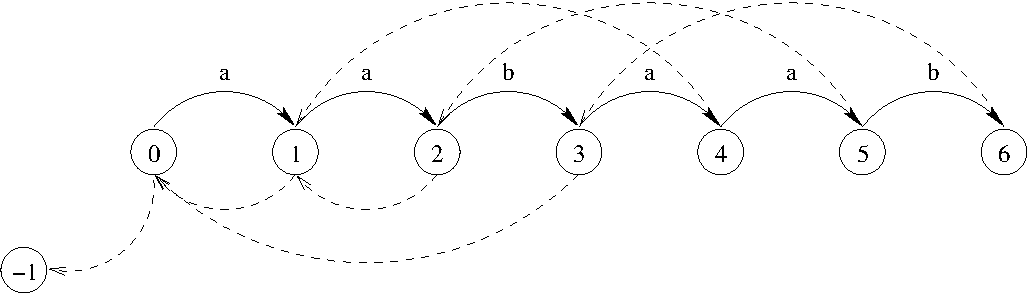
\includegraphics[scale=0.5]{./figuras/kmp.pdf}

\begin{tabular}{l|rrrrrrr}
\hline
$e$    &  0 & 1 & 2 & 3 & 4 & 5 & 6 \\
$F(e)$ & -1 & 0 & 1 & 0 & 1 & 2 & 3 \\
\hline
\end{tabular}
\caption{Aut\'omata impl\'icito en la cadena $aabaab$ (l\'ineas s\'olidas) y la funci\'on de falla $F$ (l\'ineas punteadas)}
\end{figure}

La cadena $s$ y la funci\'on de falla pueden interpretarse como un aut\'omata.
Para buscar las ocurrencias de $s$ en $t$, si se est\'a en el estado $e$ y el
caracter de entrada coincide con $s[e]$, se avanza al estado $e + 1$.
Si el caracter de entrada difiere de $s[e]$, se vuelve al estado $F(e)$
y se repite el proceso. (Si en alg\'un momento se llega al estado -1, el
caracter actual se descarta y se pasa al estado 0).

Dado que la funci\'on de falla cumple que $F(e) < e$ para todo $e$,
y que cada vez que se incrementa el estado se lee un caracter de la
entrada, la cantidad total de retrocesos no puede ser mayor que $|t|$.
Adem\'as, la construcci\'on de la tabla de $F$ es $O(|s|)$. (La
tabla se construye de la manera usual).

Por lo tanto, la complejidad temporal del algoritmo es $O(|s| + |t|)$.
La memoria utilizada es $O(|s|)$ para almacenar la tabla de $F$ y
un buffer de tama\~no constante (64 KB).

\subsection{Implementaci�n}
\noindent
\ttfamily
\shorthandoff{"}\\
\hlstd{}\hlline{\ 1\ }\hldir{\#include\ $<$vector$>$}\\
\hlline{\ 2\ }\hlstd{}\hldir{\#include\ $<$string$>$}\\
\hlline{\ 3\ }\hlstd{}\hldir{\#include\ $<$iostream$>$}\\
\hlline{\ 4\ }\hlstd{}\hldir{\#include\ $<$cassert$>$}\\
\hlline{\ 5\ }\hlstd{}\hldir{\#include\ $<$cstdlib$>$}\\
\hlline{\ 6\ }\hlstd{}\\
\hlline{\ 7\ }\hlkwa{using\ namespace\ }\hlstd{std}\hlsym{;}\\
\hlline{\ 8\ }\hlstd{}\\
\hlline{\ 9\ }\hlkwc{typedef\ }\hlstd{}\hlkwb{unsigned\ long\ long\ int\ }\hlstd{lluint}\hlsym{;}\\
\hlline{10\ }\hlstd{}\hlkwc{typedef\ }\hlstd{vector}\hlsym{$<$}\hlstd{}\hlkwb{int}\hlstd{}\hlsym{$>$\ }\hlstd{vint}\hlsym{;}\\
\hlline{11\ }\hlstd{}\\
\hlline{12\ }\hldir{\#define\ forsn(i,\ s,\ n)\ for\ (int\ i\ =\ (s);\ i\ $<$\ (n);\ i++)}\\
\hlline{13\ }\hlstd{}\hldir{\#define\ forn(i,\ n)\ forsn\ (i,\ 0,\ n)}\\
\hlline{14\ }\hlstd{}\\
\hlline{15\ }\hlslc{//\ Pre\ KMP}\\
\hlline{16\ }\hlstd{}\\
\hlline{17\ }\hlkwb{void\ }\hlstd{}\hlkwd{pkmp}\hlstd{}\hlsym{(}\hlstd{}\hlkwb{const\ }\hlstd{string}\hlsym{\&\ }\hlstd{s}\hlsym{,\ }\hlstd{vint}\hlsym{\&\ }\hlstd{f}\hlsym{)\ \{}\\
\hlline{18\ }\hlstd{\ }\hlkwb{int\ }\hlstd{z\ }\hlsym{=\ }\hlstd{f}\hlsym{{[}}\hlstd{}\hlnum{0}\hlstd{}\hlsym{{]}\ =\ {-}}\hlstd{}\hlnum{1}\hlstd{}\hlsym{;}\\
\hlline{19\ }\hlstd{\ }\hlkwd{forsn\ }\hlstd{}\hlsym{(}\hlstd{i}\hlsym{,\ }\hlstd{}\hlnum{1}\hlstd{}\hlsym{,\ }\hlstd{s}\hlsym{.}\hlstd{}\hlkwd{size}\hlstd{}\hlsym{()\ +\ }\hlstd{}\hlnum{1}\hlstd{}\hlsym{)\ \{}\\
\hlline{20\ }\hlstd{}\hlstd{\ \ }\hlstd{}\hlkwa{while\ }\hlstd{}\hlsym{(}\hlstd{z\ }\hlsym{!=\ {-}}\hlstd{}\hlnum{1\ }\hlstd{}\hlsym{\&\&\ }\hlstd{s}\hlsym{{[}}\hlstd{i\ }\hlsym{{-}\ }\hlstd{}\hlnum{1}\hlstd{}\hlsym{{]}\ !=\ }\hlstd{s}\hlsym{{[}}\hlstd{z}\hlsym{{]})\ }\hlstd{z\ }\hlsym{=\ }\hlstd{f}\hlsym{{[}}\hlstd{z}\hlsym{{]};}\\
\hlline{21\ }\hlstd{}\hlstd{\ \ }\hlstd{f}\hlsym{{[}}\hlstd{i}\hlsym{{]}\ =\ ++}\hlstd{z}\hlsym{;\ }\hlstd{}\hlslc{//\ z\ might\ be\ {-}1}\\
\hlline{22\ }\hlstd{\ }\hlsym{\}}\\
\hlline{23\ }\hlstd{}\hlsym{\}}\\
\hlline{24\ }\hlstd{}\\
\hlline{25\ }\hlslc{//\ Buffer}\\
\hlline{26\ }\hlstd{}\\
\hlline{27\ }\hldir{\#define\ TAMBUF\ 65536}\\
\hlline{28\ }\hlstd{lluint\ pos}\hlsym{;}\\
\hlline{29\ }\hlstd{}\hlkwb{char\ }\hlstd{buf}\hlsym{{[}}\hlstd{TAMBUF}\hlsym{{]};}\\
\hlline{30\ }\hlstd{}\hlkwb{int\ }\hlstd{buf\textunderscore size}\hlsym{;}\\
\hlline{31\ }\hlstd{}\\
\hlline{32\ }\hldir{\#define\ buf\textunderscore sync()\ \{\ $\backslash$}\\
\hlline{33\ }\hldir{\ cin.getline(buf,\ TAMBUF\ +\ 1);\ $\backslash$}\\
\hlline{34\ }\hldir{\ pos\ +=\ buf\textunderscore size;\ $\backslash$}\\
\hlline{35\ }\hldir{\ buf\textunderscore size\ =\ cin.gcount();\ $\backslash$}\\
\hlline{36\ }\hldir{\ cin.clear();\ $\backslash$}\\
\hlline{37\ }\hldir{\}}\\
\hlline{38\ }\hlstd{}\\
\hlline{39\ }\hldir{\#define\ buf\textunderscore start()\ \{\ $\backslash$}\\
\hlline{40\ }\hldir{\ buf\textunderscore sync();\ $\backslash$}\\
\hlline{41\ }\hldir{\ pos\ =\ 0;\ $\backslash$}\\
\hlline{42\ }\hldir{\}}\\
\hlline{43\ }\hlstd{}\\
\hlline{44\ }\hlslc{//\ KMP}\\
\hlline{45\ }\hlstd{}\\
\hlline{46\ }\hlkwb{void\ }\hlstd{}\hlkwd{kmp}\hlstd{}\hlsym{(}\hlstd{}\hlkwb{const\ }\hlstd{string}\hlsym{\&\ }\hlstd{s}\hlsym{,\ }\hlstd{vint}\hlsym{\&\ }\hlstd{f}\hlsym{)\ \{}\\
\hlline{47\ }\hlstd{\ }\hlkwd{buf\textunderscore start}\hlstd{}\hlsym{();}\\
\hlline{48\ }\hlstd{\ }\hlkwb{const\ int\ }\hlstd{final\ }\hlsym{=\ }\hlstd{s}\hlsym{.}\hlstd{}\hlkwd{size}\hlstd{}\hlsym{();}\\
\hlline{49\ }\hlstd{\ }\hlkwb{int\ }\hlstd{state\ }\hlsym{=\ }\hlstd{}\hlnum{0}\hlstd{}\hlsym{;}\\
\hlline{50\ }\hlstd{\ }\hlkwa{while\ }\hlstd{}\hlsym{(}\hlstd{}\hlkwa{true}\hlstd{}\hlsym{)\ \{}\\
\hlline{51\ }\hlstd{}\hlstd{\ \ }\hlstd{}\hlkwd{forn\ }\hlstd{}\hlsym{(}\hlstd{i}\hlsym{,\ }\hlstd{buf\textunderscore size}\hlsym{)\ \{}\\
\hlline{52\ }\hlstd{}\hlstd{\ \ \ }\hlstd{}\hlkwa{if\ }\hlstd{}\hlsym{(}\hlstd{state\ }\hlsym{==\ }\hlstd{final}\hlsym{)\ \{}\\
\hlline{53\ }\hlstd{}\hlstd{\ \ \ \ }\hlstd{cout\ }\hlsym{$<$$<$\ (}\hlstd{pos\ }\hlsym{+\ }\hlstd{i\ }\hlsym{{-}\ }\hlstd{final}\hlsym{)\ $<$$<$\ }\hlstd{}\hlstr{"\ "}\hlstd{}\hlsym{;}\\
\hlline{54\ }\hlstd{}\hlstd{\ \ \ }\hlstd{}\hlsym{\}}\\
\hlline{55\ }\hlstd{}\hlstd{\ \ \ }\hlstd{}\hlkwa{while\ }\hlstd{}\hlsym{(}\hlstd{s}\hlsym{{[}}\hlstd{state}\hlsym{{]}\ !=\ }\hlstd{buf}\hlsym{{[}}\hlstd{i}\hlsym{{]})\ \{}\\
\hlline{56\ }\hlstd{}\hlstd{\ \ \ \ }\hlstd{state\ }\hlsym{=\ }\hlstd{f}\hlsym{{[}}\hlstd{state}\hlsym{{]};}\\
\hlline{57\ }\hlstd{}\hlstd{\ \ \ \ }\hlstd{}\hlkwa{if\ }\hlstd{}\hlsym{(}\hlstd{state\ }\hlsym{==\ {-}}\hlstd{}\hlnum{1}\hlstd{}\hlsym{)\ }\hlstd{}\hlkwa{break}\hlstd{}\hlsym{;}\\
\hlline{58\ }\hlstd{}\hlstd{\ \ \ }\hlstd{}\hlsym{\}}\\
\hlline{59\ }\hlstd{}\hlstd{\ \ \ }\hlstd{state}\hlsym{++;}\\
\hlline{60\ }\hlstd{}\hlstd{\ \ }\hlstd{}\hlsym{\}}\\
\hlline{61\ }\hlstd{}\hlstd{\ \ }\hlstd{}\hlkwa{if\ }\hlstd{}\hlsym{(}\hlstd{buf\textunderscore size\ }\hlsym{$<$\ }\hlstd{TAMBUF}\hlsym{)\ }\hlstd{}\hlkwa{break}\hlstd{}\hlsym{;}\\
\hlline{62\ }\hlstd{}\hlstd{\ \ }\hlstd{}\hlkwd{buf\textunderscore sync}\hlstd{}\hlsym{();}\\
\hlline{63\ }\hlstd{\ }\hlsym{\}}\\
\hlline{64\ }\hlstd{}\hlsym{\}}\\
\hlline{65\ }\hlstd{}\\
\hlline{66\ }\hlkwb{int\ }\hlstd{}\hlkwd{main}\hlstd{}\hlsym{()\ \{}\\
\hlline{67\ }\hlstd{\ }\hlkwa{for\ }\hlstd{}\hlsym{(;;)\ \{}\\
\hlline{68\ }\hlstd{}\hlstd{\ \ }\hlstd{}\hlkwb{int\ }\hlstd{needle\textunderscore size}\hlsym{;}\\
\hlline{69\ }\hlstd{}\hlstd{\ \ }\hlstd{string\ needle}\hlsym{;}\\
\hlline{70\ }\hlstd{}\hlstd{\ \ }\hlstd{cin\ }\hlsym{$>$$>$\ }\hlstd{needle\textunderscore size}\hlsym{;}\\
\hlline{71\ }\hlstd{}\hlstd{\ \ }\hlstd{}\hlkwa{if\ }\hlstd{}\hlsym{(}\hlstd{cin}\hlsym{.}\hlstd{}\hlkwd{eof}\hlstd{}\hlsym{())\ }\hlstd{}\hlkwa{break}\hlstd{}\hlsym{;}\\
\hlline{72\ }\hlstd{}\hlstd{\ \ }\hlstd{cin\ }\hlsym{$>$$>$\ }\hlstd{needle}\hlsym{;}\\
\hlline{73\ }\hlstd{}\hlstd{\ \ }\hlstd{}\hlkwd{assert}\hlstd{}\hlsym{(}\hlstd{needle\textunderscore size\ }\hlsym{==\ }\hlstd{needle}\hlsym{.}\hlstd{}\hlkwd{size}\hlstd{}\hlsym{());}\\
\hlline{74\ }\hlstd{}\hlstd{\ \ }\hlstd{cin}\hlsym{.}\hlstd{}\hlkwd{ignore}\hlstd{}\hlsym{(}\hlstd{}\hlnum{1}\hlstd{}\hlsym{);}\\
\hlline{75\ }\hlstd{\\
\hlline{76\ }}\hlstd{\ \ }\hlstd{vint\ }\hlkwd{f}\hlstd{}\hlsym{(}\hlstd{needle}\hlsym{.}\hlstd{}\hlkwd{size}\hlstd{}\hlsym{()\ +\ }\hlstd{}\hlnum{1}\hlstd{}\hlsym{);}\\
\hlline{77\ }\hlstd{}\hlstd{\ \ }\hlstd{}\hlkwd{pkmp}\hlstd{}\hlsym{(}\hlstd{needle}\hlsym{,\ }\hlstd{f}\hlsym{);}\\
\hlline{78\ }\hlstd{}\hlstd{\ \ }\hlstd{}\hlkwd{kmp}\hlstd{}\hlsym{(}\hlstd{needle}\hlsym{,\ }\hlstd{f}\hlsym{);}\\
\hlline{79\ }\hlstd{}\hlstd{\ \ }\hlstd{cout\ }\hlsym{$<$$<$\ }\hlstd{endl}\hlsym{;}\\
\hlline{80\ }\hlstd{\ }\hlsym{\}}\\
\hlline{81\ }\hlstd{\ }\hlkwa{return\ }\hlstd{}\hlnum{0}\hlstd{}\hlsym{;}\\
\hlline{82\ }\hlstd{}\hlsym{\}}\\
\hlline{83\ }\hlstd{}\\
\mbox{}
\normalfont
\shorthandon{"}


\newcommand{\entrada}[3]{\ensuremath{[#1\text{|}#2\mapsto#3]}}

\section{3703 - Billing tables}
\textbf{Problema:}
Se tiene una tabla de entradas, cada una de las cuales describe un conjunto
de cadenas y tiene asociado un valor. Las cadenas descriptas est\'an siempre
formadas por once d\'igitos num\'ericos. Cada entrada es de
la forma $\entrada{a_1...a_k...a_n}{b_k ... b_n}{v}$
con $a_k ... a_n \leq b_k ... b_n$,
lo cual engloba a las cadenas $\{x\ |\ a_1 ... a_n \leq x \leq a_1 ... a_{k-1} b_k ... b_n\}$
(donde $\leq$~es el orden lexicogr\'afico).
El valor asociado a una cadena $s$ es el valor $v$ de la primera entrada
de la tabla que engloba a $s$.

El problema es convertir la tabla de entradas en un diccionario
equivalente (i.e. que asigne los mismos valores a las mismas cadenas).
Cada entrada del diccionario debe ser de la forma
$a_1 ... a_n \mapsto v$, lo cual asocia una cadena $s$ a $v$ sii
$a_1 ... a_n$ es prefijo de $s$. Ninguna entrada del
diccionario puede ser prefijo de otra. Adem\'as, el diccionario
debe ser m\'inimo en cantidad de entradas.

\subsection{Resoluci\'on}

\subsubsection{Representaci\'on del diccionario}

El problema se resuelve construyendo un \textit{trie} que representa
el diccionario. El \textit{trie} cumple con el siguiente invariante:

\begin{enumerate}
\item Las hojas tienen asociado un valor
\item Los nodos internos no tienen asociado un valor.
\item Todo nodo interno tiene exactamente 10 hijos (no le faltan hijos).
\item Si un nodo $x$ es interno, sea $L$ el conjunto de valores que figuran
      en el sub\'arbol cuya ra\'iz es $x$. Entonces $\#L > 1$.
      (Notar que, por la condici\'on 1, $\#L \geq 1$).
\end{enumerate}

Un \textit{trie} de estas caracter\'isticas representa un diccionario m\'inimo.
Las entradas del diccionario est\'an dadas por las ramas del \textit{trie}
y por lo tanto ninguna entrada es prefijo de otra.
Adem\'as, el diccionario $D$ es m\'inimo en cantidad de entradas.
Suponer que hubiera un diccionario $D'$ m\'as chico.
Para que $D$ y $D'$ sean equivalentes, todas las cadenas
de $D$ deben estar representadas por alguna entrada de $D'$.
Si todas las entradas de $D'$ fueran extensiones de las
entradas de $D$, entonces $D'$ tendr\'ia al menos tantas
entradas como $D$ y no ser\'ia m\'as chico.
Entonces hay al menos una entrada de $D'$ de la forma
$a_1 ... a_k \mapsto v$ que es un prefijo de alguna
entrada de $D$ de la forma $a_1 ... a_k ... a_n \mapsto v_1$.
Por la condici\'on 4, en $D$ debe haber otra entrada
$a_1 ... a_k b_{k+1} ... b_n \mapsto v_2$ con $v_1 \neq v_2$.
Por lo tanto $D$ y $D'$ no pueden ser equivalentes.

\subsubsection{Construcci\'on del diccionario a partir de la tabla}

El diccionario se construye tomando las entradas de la tabla
original y recorri\'endolas desde abajo hacia arriba.
El razonamiento inductivo es que si se tiene un diccionario $D$
equivalente a una tabla $T$, se puede construir un nuevo
diccionario $D'$ equivalente a la tabla $\entrada{a_1...a_k...a_n}{b_k...b_n}{v} \cdot T$
insertando en $D$ una cierta cantidad de elementos.
Adem\'as, el \textit{trie} de $D$ se construye respetando el invariante,
de modo tal que, por el razonamiento anterior, $D$ es m\'inimo.

Para agregar la entrada $\entrada{a_1...a_k...a_n}{b_k...b_n}{v}$,
ser\'ia posible insertar en el diccionario todas las cadenas de la forma
$a_1...a_{k-1}c_k...c_n$ tales que $a_k...a_n \leq c_k...c_n \leq b_k...b_n$.
Esto ser\'ia correcto pero potencialmente muy ineficiente.
Por ejemplo, en el peor caso, $\entrada{0^{L}}{9^{L}}{v}$
requerir\'ia insertar todas las cadenas de longitud $L$,
que es claramente exponencial en el tama\~no de la entrada.

En lugar de hacer esto, se puede insertar una cantidad de
cadenas lineal en el tama\~no de la entrada (por el tama\~no
del alfabeto, que en este caso es suficientemente chico como
para ser considerado constante).
Por ejemplo, para agregar $\entrada{7400}{499}{v}$ es redundante
insertar todos los valores intermedios $7400, 7401, 7402, \hdots, 7499$;
basta con insertar $74$. Esto es consistente con la condici\'on 4
del invariante del \textit{trie}.

En general, para agregar $\entrada{a_1...a_k...a_n}{b_k...b_n}{v}$
se insertan todas las cadenas de la forma $a_1...a_{n-1}d$ 
y todas las cadenas de la forma $a_1...a_{k-1}b_k...b_{n-1}d$
(para todo valor de $d$ que haga que dichas cadenas est\'en en el rango). Una vez hecho esto,
se aplica recursivamente el mismo procedimiento
para agregar $\entrada{a_1...a_k...a_{n-1}}{b_k...b_{n-1}}{v}$.
Esto requiere a lo sumo $n$ pasos, y en cada
paso se insertan a lo sumo $2|\Sigma|$ cadenas, siendo $|\Sigma|$ la cantidad de elementos 
del alfabeto que se utiliza.

Por ejemplo, para agregar \entrada{7377}{643}{v} se
insertan las siguientes cadenas:

\begin{itemize}
\item $7377, 7378, 7379$
\item $738, 739$
\item $74, 75$
\item $760, 761, 762, 763$
\item $7640, 7641, 7642, 7643$
\end{itemize}

El algoritmo que lista dichas cadenas se implementa
de manera iterativa, representando las cadenas de
d\'igitos como enteros de 64 bits.

\subsubsection{Modificaciones del algoritmo de inserci\'on}

Para mantener el invariante del \textit{trie}, las inserciones usan el algoritmo
habitual, con las siguientes modificaciones:

\begin{itemize}
\item Cuando se va a insertar una cadena $\alpha \beta \mapsto v$
en una hoja de la forma $\alpha \mapsto w$, se elimina el valor
$w$ de la hoja (para cumplir con la condici\'on 2, porque va a pasar
a ser un nodo interno). Se completan los hijos de la hoja, agregando
$\alpha d \mapsto w$ para todo $d \in \Sigma$ para cumplir con la
condici\'on 3. Despu\'es se prosigue insertando
$\alpha \beta \mapsto v$ en el hijo que corresponda.

\item Una vez que se insert\'o una cadena, a medida que se
va subiendo por los nodos (al volver de la recursi\'on), se
garantiza que se cumpla con la condici\'on 4 de la siguiente
manera: si todos los hijos de un nodo son hojas cuyo valor
es $v$, se eliminan todos los hijos y se etiqueta el nodo
actual con $v$. (Los hijos del nodo ya cumplen con la
condici\'on 4 del invariante; por lo tanto, si alguno de
ellos no es una hoja, hay al menos dos valores diferentes
en el sub\'arbol analizado).
\end{itemize}

\subsubsection{Complejidades}

Por lo visto arriba, en peor caso, el costo de insertar una
cadena de longitud $n$ en el \textit{trie} es $O(n |\Sigma|)$.

La complejidad total del algoritmo es la siguiente:
la tabla original tiene $k$ entradas. La $i$-\'esima
entrada describe prefijos de longitud $n_i$. Para cada
entrada, es necesario insertar a lo sumo $2 |\Sigma| n_i$
cadenas, cada una de longitud $n_i$.
En peor caso, el costo de insertar todas las cadenas asociadas
a una entrada es $O(n_i^2 |\Sigma|^2)$. %TODO: No llego a entender de donde sale esto (Fede)

El costo de insertar todas las entradas es
$O(\sum_{i=1}^{k}{n_i^2 |\Sigma|^2})$ en peor
caso. Adem\'as, se puede acotar la longitud del
prefijo por la longitud m\'axima de las cadenas:
$n_i \leq L = 11$, con lo cual el costo de insertar
todas las cadenas de una tabla es $O(k L^2 |\Sigma|^2)$.

Los valores $v$ asociados a cada entrada son cadenas
de longitud acotada (y razonablemente chica). 
Para (potencialmente) usar menos memoria y comparar
las cadenas de manera m\'as simple, se guardan en un
\texttt{set<string>} y se representan los valores
con un puntero. En una tabla de $k$ entradas hay a lo
sumo $k$ valores, y por lo tanto esto introduce un costo
adicional de $O(V \log k)$ donde $V = 20$ es la
longitud m\'axima de las cadenas que describen valores.

Por \'ultimo, el costo de iterar el diccionario e imprimirlo
es el siguiente: recorrer el \textit{trie} es lineal en la cantidad
de nodos del mismo, que es a lo sumo $O(k L^2 |\Sigma|^2)$
(resultan de insertar $O(k L |\Sigma|)$ cadenas, cada una de las
cuales agrega como mucho $O(L |\Sigma|)$ nodos).
Para cada hoja, se imprime el prefijo que le corresponde
al nodo en cuesti\'on, de largo $L$, y el valor asociado, de largo $V$.

Notando que $V \in O(L)$ y que el costo de mantener el conjunto
de cadenas $O(V \log k)$ est\'a inclu\'ido en el costo de las
dem\'as operaciones, el costo total en peor caso es
$O(k L^3 |\Sigma|^2)$.
Si se desprecian las constantes $L = 11$, $|\Sigma| = 10$ por
ser $O(1)$, la complejidad en peor caso es $O(k)$.

\subsection{Implementaci�n}
\noindent
\ttfamily
\shorthandoff{"}\\
\hlstd{}\hlline{\ 1\ }\hldir{\#include\ $<$string$>$}\\
\hlline{\ 2\ }\hlstd{}\hldir{\#include\ $<$map$>$}\\
\hlline{\ 3\ }\hlstd{}\hldir{\#include\ $<$set$>$}\\
\hlline{\ 4\ }\hlstd{}\hldir{\#include\ $<$vector$>$}\\
\hlline{\ 5\ }\hlstd{}\hldir{\#include\ $<$stack$>$}\\
\hlline{\ 6\ }\hlstd{}\hldir{\#include\ $<$iostream$>$}\\
\hlline{\ 7\ }\hlstd{}\hldir{\#include\ $<$sstream$>$}\\
\hlline{\ 8\ }\hlstd{}\hldir{\#include\ $<$iomanip$>$}\\
\hlline{\ 9\ }\hlstd{}\hldir{\#include\ $<$cassert$>$}\\
\hlline{10\ }\hlstd{}\hldir{\#include\ $<$cstdlib$>$}\\
\hlline{11\ }\hlstd{}\hldir{\#include\ $<$stdio.h$>$}\\
\hlline{12\ }\hlstd{}\\
\hlline{13\ }\hlkwa{using\ namespace\ }\hlstd{std}\hlsym{;}\\
\hlline{14\ }\hlstd{}\\
\hlline{15\ }\hldir{\#define\ forsn(i,\ s,\ n)\ for\ (int\ i\ =\ (s);\ i\ $<$\ (n);\ i++)}\\
\hlline{16\ }\hlstd{}\hldir{\#define\ forn(i,\ n)\ forsn\ (i,\ 0,\ n)}\\
\hlline{17\ }\hlstd{}\hldir{\#define\ dforn(i,\ n)\ for\ (int\ i\ =\ (n);\ i{-}{-}\ $>$\ 0;)}\\
\hlline{18\ }\hlstd{}\\
\hlline{19\ }\hldir{\#define\ ALPHA\textunderscore SIZE\ 10}\\
\hlline{20\ }\hlstd{}\hldir{\#define\ ALPHA\textunderscore VAL(C)\ ((C)\ {-}\ }\hldstr{`0`}\hldir{)}\\
\hlline{21\ }\hlstd{}\hldir{\#define\ foralpha(x)\ forn\ (x,\ ALPHA\textunderscore SIZE)}\\
\hlline{22\ }\hlstd{}\\
\hlline{23\ }\hlkwc{typedef\ }\hlstd{}\hlkwb{unsigned\ long\ long\ int\ }\hlstd{lluint}\hlsym{;}\\
\hlline{24\ }\hlstd{}\\
\hlline{25\ }\hlkwc{typedef\ }\hlstd{}\hlkwb{const\ }\hlstd{string\ }\hlsym{{*}}\hlstd{Value}\hlsym{;}\\
\hlline{26\ }\hlstd{\\
\hlline{27\ }string\ }\hlkwd{itos}\hlstd{}\hlsym{(}\hlstd{lluint\ i}\hlsym{,\ }\hlstd{}\hlkwb{int\ }\hlstd{width}\hlsym{)\ \{}\\
\hlline{28\ }\hlstd{\ }\hlkwa{if\ }\hlstd{}\hlsym{(}\hlstd{width\ }\hlsym{==\ }\hlstd{}\hlnum{0}\hlstd{}\hlsym{)\ }\hlstd{}\hlkwa{return\ }\hlstd{}\hlstr{``''}\hlstd{}\hlsym{;}\\
\hlline{29\ }\hlstd{\ ostringstream\ os}\hlsym{;}\\
\hlline{30\ }\hlstd{\ os\ }\hlsym{$<$$<$\ }\hlstd{}\hlkwd{setw}\hlstd{}\hlsym{(}\hlstd{width}\hlsym{)\ $<$$<$\ }\hlstd{}\hlkwd{setfill}\hlstd{}\hlsym{(}\hlstd{}\hlstr{`0`}\hlstd{}\hlsym{)\ $<$$<$\ }\hlstd{i}\hlsym{;}\\
\hlline{31\ }\hlstd{\ }\hlkwa{return\ }\hlstd{os}\hlsym{.}\hlstd{}\hlkwd{str}\hlstd{}\hlsym{();}\\
\hlline{32\ }\hlstd{}\hlsym{\}}\\
\hlline{33\ }\hlstd{}\\
\hlline{34\ }\hlcom{/{*}{*}{*}{*}\ String\ register\ {*}{*}{*}{*}/}\hlstd{\\
\hlline{35\ }\\
\hlline{36\ }set}\hlsym{$<$}\hlstd{string}\hlsym{$>$\ }\hlstd{\textunderscore reg}\hlsym{;}\\
\hlline{37\ }\hlstd{\\
\hlline{38\ }Value\ }\hlkwd{reg\textunderscore intern}\hlstd{}\hlsym{(}\hlstd{}\hlkwb{const\ }\hlstd{string}\hlsym{\&\ }\hlstd{s}\hlsym{)\ \{}\\
\hlline{39\ }\hlstd{\ }\hlkwa{return\ }\hlstd{}\hlsym{\&{*}}\hlstd{\textunderscore reg}\hlsym{.}\hlstd{}\hlkwd{insert}\hlstd{}\hlsym{(}\hlstd{s}\hlsym{).}\hlstd{first}\hlsym{;}\\
\hlline{40\ }\hlstd{}\hlsym{\}}\\
\hlline{41\ }\hlstd{}\\
\hlline{42\ }\hlkwb{void\ }\hlstd{}\hlkwd{reg\textunderscore free}\hlstd{}\hlsym{()\ \{}\\
\hlline{43\ }\hlstd{\ \textunderscore reg\ }\hlsym{=\ }\hlstd{set}\hlsym{$<$}\hlstd{string}\hlsym{$>$();}\\
\hlline{44\ }\hlstd{}\hlsym{\}}\\
\hlline{45\ }\hlstd{}\\
\hlline{46\ }\hlcom{/{*}{*}{*}{*}\ Trie\ {*}{*}{*}{*}/}\hlstd{}\\
\hlline{47\ }\\
\hlline{48\ }\hlkwb{struct\ }\hlstd{Node\ }\hlsym{\{}\\
\hlline{49\ }\hlstd{\ Node\ }\hlsym{{*}}\hlstd{children}\hlsym{{[}}\hlstd{ALPHA\textunderscore SIZE}\hlsym{{]};}\\
\hlline{50\ }\hlstd{\ Value\ value}\hlsym{;}\\
\hlline{51\ }\hlstd{}\hlsym{\};}\\
\hlline{52\ }\hlstd{}\\
\hlline{53\ }\hlkwc{typedef\ }\hlstd{Node\ }\hlsym{{*}}\hlstd{Trie}\hlsym{;}\\
\hlline{54\ }\hlstd{}\hldir{\#define\ trie\textunderscore new()\ NULL}\\
\hlline{55\ }\hlstd{}\hldir{\#define\ Empty}\hlstd{\ \ }\hldir{NULL}\\
\hlline{56\ }\hlstd{}\\
\hlline{57\ }\hlkwb{void\ }\hlstd{}\hlkwd{trie\textunderscore free}\hlstd{}\hlsym{(}\hlstd{Trie\ tr}\hlsym{)\ \{}\\
\hlline{58\ }\hlstd{\ }\hlkwa{if\ }\hlstd{}\hlsym{(!}\hlstd{tr}\hlsym{)\ }\hlstd{}\hlkwa{return}\hlstd{}\hlsym{;}\\
\hlline{59\ }\hlstd{\ }\hlkwd{foralpha\ }\hlstd{}\hlsym{(}\hlstd{dig}\hlsym{)\ \{}\\
\hlline{60\ }\hlstd{}\hlstd{\ \ }\hlstd{}\hlkwd{trie\textunderscore free}\hlstd{}\hlsym{(}\hlstd{tr}\hlsym{{-}$>$}\hlstd{children}\hlsym{{[}}\hlstd{dig}\hlsym{{]});}\\
\hlline{61\ }\hlstd{\ }\hlsym{\}}\\
\hlline{62\ }\hlstd{\ }\hlkwa{delete\ }\hlstd{tr}\hlsym{;}\\
\hlline{63\ }\hlstd{}\hlsym{\}}\\
\hlline{64\ }\hlstd{}\\
\hlline{65\ }\hlkwb{void\ }\hlstd{}\hlkwd{\textunderscore trie\textunderscore delete\textunderscore children}\hlstd{}\hlsym{(}\hlstd{Trie\ tr}\hlsym{)\ \{}\\
\hlline{66\ }\hlstd{\ }\hlkwd{foralpha\ }\hlstd{}\hlsym{(}\hlstd{dig}\hlsym{)\ }\hlstd{}\hlkwa{if\ }\hlstd{}\hlsym{(}\hlstd{tr}\hlsym{{-}$>$}\hlstd{children}\hlsym{{[}}\hlstd{dig}\hlsym{{]})\ \{}\\
\hlline{67\ }\hlstd{}\hlstd{\ \ }\hlstd{}\hlkwd{trie\textunderscore free}\hlstd{}\hlsym{(}\hlstd{tr}\hlsym{{-}$>$}\hlstd{children}\hlsym{{[}}\hlstd{dig}\hlsym{{]});}\\
\hlline{68\ }\hlstd{}\hlstd{\ \ }\hlstd{tr}\hlsym{{-}$>$}\hlstd{children}\hlsym{{[}}\hlstd{dig}\hlsym{{]}\ =\ }\hlstd{NULL}\hlsym{;}\\
\hlline{69\ }\hlstd{\ }\hlsym{\}}\\
\hlline{70\ }\hlstd{}\hlsym{\}}\\
\hlline{71\ }\hlstd{}\\
\hlline{72\ }\hlkwb{void\ }\hlstd{}\hlkwd{\textunderscore trie\textunderscore collapse\textunderscore children}\hlstd{}\hlsym{(}\hlstd{Trie\ tr}\hlsym{)\ \{}\\
\hlline{73\ }\hlstd{\ }\hlkwa{if\ }\hlstd{}\hlsym{(!}\hlstd{tr}\hlsym{{-}$>$}\hlstd{children}\hlsym{{[}}\hlstd{}\hlnum{0}\hlstd{}\hlsym{{]}\ \textbar \textbar \ }\hlstd{tr}\hlsym{{-}$>$}\hlstd{children}\hlsym{{[}}\hlstd{}\hlnum{0}\hlstd{}\hlsym{{]}{-}$>$}\hlstd{value\ }\hlsym{==\ }\hlstd{Empty}\hlsym{)\ }\hlstd{}\hlkwa{return}\hlstd{}\hlsym{;}\\
\hlline{74\ }\hlstd{\ }\hlkwd{foralpha\ }\hlstd{}\hlsym{(}\hlstd{dig}\hlsym{)\ \{}\\
\hlline{75\ }\hlstd{}\hlstd{\ \ }\hlstd{}\hlkwa{if\ }\hlstd{}\hlsym{(!}\hlstd{tr}\hlsym{{-}$>$}\hlstd{children}\hlsym{{[}}\hlstd{dig}\hlsym{{]})\ }\hlstd{}\hlkwa{return}\hlstd{}\hlsym{;}\\
\hlline{76\ }\hlstd{}\hlstd{\ \ }\hlstd{}\hlkwa{if\ }\hlstd{}\hlsym{(}\hlstd{tr}\hlsym{{-}$>$}\hlstd{children}\hlsym{{[}}\hlstd{dig}\hlsym{{]}{-}$>$}\hlstd{value\ }\hlsym{!=\ }\hlstd{tr}\hlsym{{-}$>$}\hlstd{children}\hlsym{{[}}\hlstd{}\hlnum{0}\hlstd{}\hlsym{{]}{-}$>$}\hlstd{value}\hlsym{)\ }\hlstd{}\hlkwa{return}\hlstd{}\hlsym{;}\\
\hlline{77\ }\hlstd{\ }\hlsym{\}}\\
\hlline{78\ }\hlstd{\\
\hlline{79\ }\ tr}\hlsym{{-}$>$}\hlstd{value\ }\hlsym{=\ }\hlstd{tr}\hlsym{{-}$>$}\hlstd{children}\hlsym{{[}}\hlstd{}\hlnum{0}\hlstd{}\hlsym{{]}{-}$>$}\hlstd{value}\hlsym{;}\\
\hlline{80\ }\hlstd{\ }\hlkwd{\textunderscore trie\textunderscore delete\textunderscore children}\hlstd{}\hlsym{(}\hlstd{tr}\hlsym{);}\\
\hlline{81\ }\hlstd{}\hlsym{\}}\\
\hlline{82\ }\hlstd{}\\
\hlline{83\ }\hlslc{//\ invariante:\ los\ valores\ estan\ en\ las\ hojas}\\
\hlline{84\ }\hlstd{}\hlkwb{void\ }\hlstd{}\hlkwd{trie\textunderscore add}\hlstd{}\hlsym{(}\hlstd{Trie\ }\hlsym{{*}}\hlstd{tr}\hlsym{,\ }\hlstd{}\hlkwb{const\ char\ }\hlstd{}\hlsym{{*}}\hlstd{s}\hlsym{,\ }\hlstd{Value\ v}\hlsym{)\ \{}\\
\hlline{85\ }\hlstd{\ }\hlkwa{if\ }\hlstd{}\hlsym{({*}}\hlstd{tr\ }\hlsym{==\ }\hlstd{NULL}\hlsym{)\ \{}\\
\hlline{86\ }\hlstd{}\hlstd{\ \ }\hlstd{}\hlsym{{*}}\hlstd{tr\ }\hlsym{=\ }\hlstd{}\hlkwa{new\ }\hlstd{}\hlkwd{Node}\hlstd{}\hlsym{();}\\
\hlline{87\ }\hlstd{}\hlstd{\ \ }\hlstd{}\hlkwd{foralpha\ }\hlstd{}\hlsym{(}\hlstd{dig}\hlsym{)\ ({*}}\hlstd{tr}\hlsym{){-}$>$}\hlstd{children}\hlsym{{[}}\hlstd{dig}\hlsym{{]}\ =\ }\hlstd{NULL}\hlsym{;}\\
\hlline{88\ }\hlstd{}\hlstd{\ \ }\hlstd{}\hlsym{({*}}\hlstd{tr}\hlsym{){-}$>$}\hlstd{value\ }\hlsym{=\ }\hlstd{Empty}\hlsym{;}\\
\hlline{89\ }\hlstd{\ }\hlsym{\}}\\
\hlline{90\ }\hlstd{\ }\hlkwa{if\ }\hlstd{}\hlsym{(!{*}}\hlstd{s}\hlsym{)\ \{}\\
\hlline{91\ }\hlstd{}\hlstd{\ \ }\hlstd{}\hlsym{({*}}\hlstd{tr}\hlsym{){-}$>$}\hlstd{value\ }\hlsym{=\ }\hlstd{v}\hlsym{;}\\
\hlline{92\ }\hlstd{}\hlstd{\ \ }\hlstd{}\hlkwd{\textunderscore trie\textunderscore delete\textunderscore children}\hlstd{}\hlsym{({*}}\hlstd{tr}\hlsym{);}\\
\hlline{93\ }\hlstd{\ }\hlsym{\}\ }\hlstd{}\hlkwa{else\ }\hlstd{}\hlsym{\{}\\
\hlline{94\ }\hlstd{}\hlstd{\ \ }\hlstd{}\hlkwa{if\ }\hlstd{}\hlsym{(({*}}\hlstd{tr}\hlsym{){-}$>$}\hlstd{value\ }\hlsym{!=\ }\hlstd{Empty}\hlsym{)\ \{}\\
\hlline{95\ }\hlstd{}\hlstd{\ \ \ }\hlstd{}\hlkwd{foralpha\ }\hlstd{}\hlsym{(}\hlstd{dig}\hlsym{)\ \{}\\
\hlline{96\ }\hlstd{}\hlstd{\ \ \ \ }\hlstd{}\hlkwd{trie\textunderscore add}\hlstd{}\hlsym{(\&({*}}\hlstd{tr}\hlsym{){-}$>$}\hlstd{children}\hlsym{{[}}\hlstd{dig}\hlsym{{]},\ }\hlstd{}\hlstr{""}\hlstd{}\hlsym{,\ ({*}}\hlstd{tr}\hlsym{){-}$>$}\hlstd{value}\hlsym{);}\\
\hlline{97\ }\hlstd{}\hlstd{\ \ \ }\hlstd{}\hlsym{\}}\\
\hlline{98\ }\hlstd{}\hlstd{\ \ \ }\hlstd{}\hlsym{({*}}\hlstd{tr}\hlsym{){-}$>$}\hlstd{value\ }\hlsym{=\ }\hlstd{Empty}\hlsym{;}\\
\hlline{99\ }\hlstd{}\hlstd{\ \ }\hlstd{}\hlsym{\}}\\
\hlline{100\ }\hlstd{}\hlstd{\ \ }\hlstd{}\hlkwd{trie\textunderscore add}\hlstd{}\hlsym{(\&({*}}\hlstd{tr}\hlsym{){-}$>$}\hlstd{children}\hlsym{{[}}\hlstd{}\hlkwd{ALPHA\textunderscore VAL}\hlstd{}\hlsym{({*}}\hlstd{s}\hlsym{){]},\ \&}\hlstd{s}\hlsym{{[}}\hlstd{}\hlnum{1}\hlstd{}\hlsym{{]},\ }\hlstd{v}\hlsym{);}\\
\hlline{101\ }\hlstd{\\
\hlline{102\ }}\hlstd{\ \ }\hlstd{}\hlkwd{\textunderscore trie\textunderscore collapse\textunderscore children}\hlstd{}\hlsym{({*}}\hlstd{tr}\hlsym{);}\\
\hlline{103\ }\hlstd{\ }\hlsym{\}}\\
\hlline{104\ }\hlstd{}\hlsym{\}}\\
\hlline{105\ }\hlstd{}\\
\hlline{106\ }\hlkwb{bool\ }\hlstd{}\hlkwd{trie\textunderscore has\textunderscore children}\hlstd{}\hlsym{(}\hlstd{Trie\ tr}\hlsym{)\ \{}\\
\hlline{107\ }\hlstd{\ }\hlkwd{foralpha\ }\hlstd{}\hlsym{(}\hlstd{dig}\hlsym{)\ \{}\\
\hlline{108\ }\hlstd{}\hlstd{\ \ }\hlstd{}\hlkwa{if\ }\hlstd{}\hlsym{(}\hlstd{tr}\hlsym{{-}$>$}\hlstd{children}\hlsym{{[}}\hlstd{dig}\hlsym{{]}\ ==\ }\hlstd{NULL}\hlsym{)\ }\hlstd{}\hlkwa{continue}\hlstd{}\hlsym{;}\\
\hlline{109\ }\hlstd{}\hlstd{\ \ }\hlstd{}\hlkwa{return\ true}\hlstd{}\hlsym{;}\\
\hlline{110\ }\hlstd{\ }\hlsym{\}}\\
\hlline{111\ }\hlstd{\ }\hlkwa{return\ false}\hlstd{}\hlsym{;}\\
\hlline{112\ }\hlstd{}\hlsym{\}}\\
\hlline{113\ }\hlstd{}\\
\hlline{114\ }\hlkwb{void\ }\hlstd{}\hlkwd{trie\textunderscore debug}\hlstd{}\hlsym{(}\hlstd{Trie\ tr}\hlsym{,\ }\hlstd{}\hlkwb{int\ }\hlstd{depth}\hlsym{)\ \{}\\
\hlline{115\ }\hlstd{\ }\hlkwa{if\ }\hlstd{}\hlsym{(!}\hlstd{tr}\hlsym{)\ }\hlstd{}\hlkwa{return}\hlstd{}\hlsym{;}\\
\hlline{116\ }\hlstd{\ }\hlkwd{foralpha\ }\hlstd{}\hlsym{(}\hlstd{dig}\hlsym{)\ \{}\\
\hlline{117\ }\hlstd{}\hlstd{\ \ }\hlstd{}\hlkwa{if\ }\hlstd{}\hlsym{(!}\hlstd{tr}\hlsym{{-}$>$}\hlstd{children}\hlsym{{[}}\hlstd{dig}\hlsym{{]})\ }\hlstd{}\hlkwa{continue}\hlstd{}\hlsym{;}\\
\hlline{118\ }\hlstd{}\hlstd{\ \ }\hlstd{}\hlkwd{forn\ }\hlstd{}\hlsym{(}\hlstd{i}\hlsym{,\ }\hlstd{depth}\hlsym{)\ \{\ }\hlstd{cout\ }\hlsym{$<$$<$\ }\hlstd{}\hlstr{``\ }\hlstd{}\hlsym{;\ \}}\\
\hlline{119\ }\hlstd{}\hlstd{\ \ }\hlstd{cout\ }\hlsym{$<$$<$\ }\hlstd{}\hlkwd{itos}\hlstd{}\hlsym{(}\hlstd{dig}\hlsym{,\ }\hlstd{}\hlnum{1}\hlstd{}\hlsym{);}\\
\hlline{120\ }\hlstd{}\hlstd{\ \ }\hlstd{}\hlkwa{if\ }\hlstd{}\hlsym{(}\hlstd{tr}\hlsym{{-}$>$}\hlstd{children}\hlsym{{[}}\hlstd{dig}\hlsym{{]}{-}$>$}\hlstd{value}\hlsym{)\ \{}\\
\hlline{121\ }\hlstd{}\hlstd{\ \ \ }\hlstd{cout\ }\hlsym{$<$$<$\ }\hlstd{}\hlstr{"}\hlstd{\ \ }\hlstr{("}\hlstd{\ }\hlsym{$<$$<$\ {*}(}\hlstd{tr}\hlsym{{-}$>$}\hlstd{children}\hlsym{{[}}\hlstd{dig}\hlsym{{]}{-}$>$}\hlstd{value}\hlsym{)\ $<$$<$\ }\hlstd{}\hlstr{")"}\hlstd{}\hlsym{;}\\
\hlline{122\ }\hlstd{}\hlstd{\ \ }\hlstd{}\hlsym{\}}\\
\hlline{123\ }\hlstd{}\hlstd{\ \ }\hlstd{cout\ }\hlsym{$<$$<$\ }\hlstd{endl}\hlsym{;}\\
\hlline{124\ }\hlstd{}\hlstd{\ \ }\hlstd{}\hlkwd{trie\textunderscore debug}\hlstd{}\hlsym{(}\hlstd{tr}\hlsym{{-}$>$}\hlstd{children}\hlsym{{[}}\hlstd{dig}\hlsym{{]},\ }\hlstd{depth\ }\hlsym{+\ }\hlstd{}\hlnum{1}\hlstd{}\hlsym{);}\\
\hlline{125\ }\hlstd{\ }\hlsym{\}}\\
\hlline{126\ }\hlstd{}\hlsym{\}}\\
\hlline{127\ }\hlstd{}\\
\hlline{128\ }\hlcom{/{*}{*}{*}{*}\ Resultado\ {*}{*}{*}{*}/}\hlstd{}\\
\hlline{129\ }\\
\hlline{130\ }\hlkwc{typedef\ }\hlstd{pair}\hlsym{$<$}\hlstd{string}\hlsym{,\ }\hlstd{Value}\hlsym{$>$\ }\hlstd{ResultItem}\hlsym{;}\\
\hlline{131\ }\hlstd{vector}\hlsym{$<$}\hlstd{ResultItem}\hlsym{$>$\ }\hlstd{result}\hlsym{;}\\
\hlline{132\ }\hlstd{Value\ Invalid}\hlsym{;}\\
\hlline{133\ }\hlstd{}\\
\hlline{134\ }\hldir{\#define\ \textunderscore produce(S,\ V)}\hlstd{\ \ }\hldir{if\ ((V)\ !=\ Invalid)\ \{\ result.push\textunderscore back(ResultItem((S),\ (V)));\ \}}\\
\hlline{135\ }\hlstd{}\hldir{\#define\ Maxlen\ 20}\\
\hlline{136\ }\hlstd{}\hlkwb{char\ }\hlstd{prefix\textunderscore buf}\hlsym{{[}}\hlstd{Maxlen}\hlsym{{]};}\\
\hlline{137\ }\hlstd{}\hlkwb{void\ }\hlstd{}\hlkwd{\textunderscore build\textunderscore result\textunderscore rec}\hlstd{}\hlsym{(}\hlstd{Trie\ tr}\hlsym{,\ }\hlstd{}\hlkwb{int\ }\hlstd{prefix\textunderscore length}\hlsym{)\ \{}\\
\hlline{138\ }\hlstd{\ }\hlkwa{if\ }\hlstd{}\hlsym{(}\hlstd{tr\ }\hlsym{==\ }\hlstd{NULL}\hlsym{)\ }\hlstd{}\hlkwa{return}\hlstd{}\hlsym{;}\\
\hlline{139\ }\hlstd{\ }\hlkwa{if\ }\hlstd{}\hlsym{(!}\hlstd{}\hlkwd{trie\textunderscore has\textunderscore children}\hlstd{}\hlsym{(}\hlstd{tr}\hlsym{))\ \{}\\
\hlline{140\ }\hlstd{}\hlstd{\ \ }\hlstd{}\hlslc{//\ no\ children}\\
\hlline{141\ }\hlstd{}\hlstd{\ \ }\hlstd{prefix\textunderscore buf}\hlsym{{[}}\hlstd{prefix\textunderscore length}\hlsym{{]}\ =\ }\hlstd{}\hlstr{`$\backslash$0`}\hlstd{}\hlsym{;}\\
\hlline{142\ }\hlstd{}\hlstd{\ \ }\hlstd{}\hlkwd{\textunderscore produce}\hlstd{}\hlsym{(}\hlstd{}\hlkwd{string}\hlstd{}\hlsym{(}\hlstd{prefix\textunderscore buf}\hlsym{),\ }\hlstd{tr}\hlsym{{-}$>$}\hlstd{value}\hlsym{);}\\
\hlline{143\ }\hlstd{\ }\hlsym{\}\ }\hlstd{}\hlkwa{else\ }\hlstd{}\hlsym{\{}\\
\hlline{144\ }\hlstd{}\hlstd{\ \ }\hlstd{}\hlslc{//\ visit\ the\ children}\\
\hlline{145\ }\hlstd{}\hlstd{\ \ }\hlstd{}\hlkwd{foralpha\ }\hlstd{}\hlsym{(}\hlstd{dig}\hlsym{)\ \{}\\
\hlline{146\ }\hlstd{}\hlstd{\ \ \ }\hlstd{prefix\textunderscore buf}\hlsym{{[}}\hlstd{prefix\textunderscore length}\hlsym{{]}\ =\ }\hlstd{}\hlstr{`0`}\hlstd{\ }\hlsym{+\ }\hlstd{dig}\hlsym{;}\\
\hlline{147\ }\hlstd{}\hlstd{\ \ \ }\hlstd{}\hlkwd{\textunderscore build\textunderscore result\textunderscore rec}\hlstd{}\hlsym{(}\hlstd{tr}\hlsym{{-}$>$}\hlstd{children}\hlsym{{[}}\hlstd{dig}\hlsym{{]},\ }\hlstd{prefix\textunderscore length\ }\hlsym{+\ }\hlstd{}\hlnum{1}\hlstd{}\hlsym{);}\\
\hlline{148\ }\hlstd{}\hlstd{\ \ }\hlstd{}\hlsym{\}}\\
\hlline{149\ }\hlstd{\ }\hlsym{\}}\\
\hlline{150\ }\hlstd{}\hlsym{\}}\\
\hlline{151\ }\hlstd{}\\
\hlline{152\ }\hlkwb{void\ }\hlstd{}\hlkwd{trie\textunderscore print\textunderscore result}\hlstd{}\hlsym{(}\hlstd{Trie\ tr}\hlsym{)\ \{}\\
\hlline{153\ }\hlstd{\ Invalid\ }\hlsym{=\ }\hlstd{}\hlkwd{reg\textunderscore intern}\hlstd{}\hlsym{(}\hlstd{}\hlstr{"invalid"}\hlstd{}\hlsym{);}\\
\hlline{154\ }\hlstd{\ result\ }\hlsym{=\ }\hlstd{vector}\hlsym{$<$}\hlstd{ResultItem}\hlsym{$>$();}\\
\hlline{155\ }\hlstd{\\
\hlline{156\ }\ }\hlkwa{if\ }\hlstd{}\hlsym{(!}\hlstd{}\hlkwd{trie\textunderscore has\textunderscore children}\hlstd{}\hlsym{(}\hlstd{tr}\hlsym{)\ \&\&\ }\hlstd{tr}\hlsym{{-}$>$}\hlstd{value\ }\hlsym{!=\ }\hlstd{Empty\ }\hlsym{\&\&\ }\hlstd{tr}\hlsym{{-}$>$}\hlstd{value\ }\hlsym{!=\ }\hlstd{Invalid}\hlsym{)\ \{}\\
\hlline{157\ }\hlstd{}\hlstd{\ \ }\hlstd{}\hlslc{//\ special\ case:\ every\ prefix\ has\ the\ same\ type}\\
\hlline{158\ }\hlstd{}\hlstd{\ \ }\hlstd{}\hlkwd{printf}\hlstd{}\hlsym{(}\hlstd{}\hlstr{"\%d}\hlesc{$\backslash$n}\hlstr{"}\hlstd{}\hlsym{,}\hlstd{ALPHA\textunderscore SIZE}\hlsym{);}\\
\hlline{159\ }\hlstd{}\hlstd{\ \ }\hlstd{}\hlkwd{foralpha\ }\hlstd{}\hlsym{(}\hlstd{dig}\hlsym{)\ \{}\\
\hlline{160\ }\hlstd{}\hlstd{\ \ \ }\hlstd{}\hlkwd{printf}\hlstd{}\hlsym{(}\hlstd{}\hlstr{"\%d\ \%s}\hlesc{$\backslash$n}\hlstr{"}\hlstd{}\hlsym{,}\hlstd{dig}\hlsym{,({*}}\hlstd{tr}\hlsym{{-}$>$}\hlstd{value}\hlsym{).}\hlstd{}\hlkwd{c\textunderscore str}\hlstd{}\hlsym{());}\\
\hlline{161\ }\hlstd{}\hlstd{\ \ }\hlstd{}\hlsym{\}}\\
\hlline{162\ }\hlstd{\ }\hlsym{\}\ }\hlstd{}\hlkwa{else\ }\hlstd{}\hlsym{\{}\\
\hlline{163\ }\hlstd{}\hlstd{\ \ }\hlstd{}\hlkwd{\textunderscore build\textunderscore result\textunderscore rec}\hlstd{}\hlsym{(}\hlstd{tr}\hlsym{,\ }\hlstd{}\hlnum{0}\hlstd{}\hlsym{);}\\
\hlline{164\ }\hlstd{\\
\hlline{165\ }}\hlstd{\ \ }\hlstd{}\hlkwd{printf}\hlstd{}\hlsym{(}\hlstd{}\hlstr{"\%d}\hlesc{$\backslash$n}\hlstr{"}\hlstd{}\hlsym{,}\hlstd{result}\hlsym{.}\hlstd{}\hlkwd{size}\hlstd{}\hlsym{());}\\
\hlline{166\ }\hlstd{}\hlstd{\ \ }\hlstd{}\hlkwd{forn\ }\hlstd{}\hlsym{(}\hlstd{i}\hlsym{,\ (}\hlstd{}\hlkwb{int}\hlstd{}\hlsym{)}\hlstd{result}\hlsym{.}\hlstd{}\hlkwd{size}\hlstd{}\hlsym{())\ \{}\\
\hlline{167\ }\hlstd{}\hlstd{\ \ \ }\hlstd{}\hlkwd{printf}\hlstd{}\hlsym{(}\hlstd{}\hlstr{"\%s\ \%s}\hlesc{$\backslash$n}\hlstr{"}\hlstd{}\hlsym{,}\hlstd{result}\hlsym{{[}}\hlstd{i}\hlsym{{]}.}\hlstd{first}\hlsym{.}\hlstd{}\hlkwd{c\textunderscore str}\hlstd{}\hlsym{(),({*}}\hlstd{result}\hlsym{{[}}\hlstd{i}\hlsym{{]}.}\hlstd{second}\hlsym{).}\hlstd{}\hlkwd{c\textunderscore str}\hlstd{}\hlsym{());}\\
\hlline{168\ }\hlstd{}\hlstd{\ \ }\hlstd{}\hlsym{\}}\\
\hlline{169\ }\hlstd{\ }\hlsym{\}}\\
\hlline{170\ }\hlstd{}\hlsym{\}}\\
\hlline{171\ }\hlstd{}\\
\hlline{172\ }\hlcom{/{*}{*}{*}{*}\ Intervalos\ {*}{*}{*}{*}/}\hlstd{}\\
\hlline{173\ }\\
\hlline{174\ }\hldir{\#define\ IMP(X,\ Y)\ (!(X)\ \textbar \textbar \ (Y))}\\
\hlline{175\ }\hlstd{}\hlkwb{void\ }\hlstd{}\hlkwd{add\textunderscore interval}\hlstd{}\hlsym{(}\hlstd{Trie\ }\hlsym{{*}}\hlstd{tr}\hlsym{,\ }\hlstd{}\hlkwb{int\ }\hlstd{pref\textunderscore size}\hlsym{,\ }\hlstd{lluint\ from}\hlsym{,\ }\hlstd{lluint\ to}\hlsym{,\ }\hlstd{Value\ val}\hlsym{)\ \{}\\
\hlline{176\ }\hlstd{\ lluint\ pot\ }\hlsym{=\ }\hlstd{}\hlnum{1}\hlstd{}\hlsym{;}\\
\hlline{177\ }\hlstd{\ }\hlkwd{forn\ }\hlstd{}\hlsym{(}\hlstd{t}\hlsym{,\ }\hlstd{}\hlnum{2}\hlstd{}\hlsym{)\ \{}\\
\hlline{178\ }\hlstd{}\hlstd{\ \ }\hlstd{lluint\ }\hlsym{{*}}\hlstd{from\textunderscore to\ }\hlsym{=\ (}\hlstd{t\ }\hlsym{==\ }\hlstd{}\hlnum{0\ }\hlstd{?\ }\hlsym{\&}\hlstd{from\ }\hlsym{:\ \&}\hlstd{to}\hlsym{);}\\
\hlline{179\ }\hlstd{}\hlstd{\ \ }\hlstd{}\hlkwa{while\ }\hlstd{}\hlsym{(}\hlstd{pot\ }\hlsym{$>$\ }\hlstd{}\hlnum{0\ }\hlstd{}\hlsym{\&\&\ }\hlstd{}\hlkwd{IMP}\hlstd{}\hlsym{(}\hlstd{t\ }\hlsym{==\ }\hlstd{}\hlnum{0}\hlstd{}\hlsym{,\ }\hlstd{from\ }\hlsym{+\ }\hlstd{pot\ }\hlsym{$<$=\ }\hlstd{to}\hlsym{))\ \{}\\
\hlline{180\ }\hlstd{}\hlstd{\ \ \ }\hlstd{}\hlkwa{while\ }\hlstd{}\hlsym{(}\hlstd{from\ }\hlsym{+\ }\hlstd{pot\ }\hlsym{$<$=\ }\hlstd{to\ }\hlsym{\&\&\ {*}}\hlstd{from\textunderscore to\ }\hlsym{\%\ (}\hlstd{pot\ }\hlsym{{*}\ }\hlstd{}\hlnum{10}\hlstd{}\hlsym{)\ $>$\ }\hlstd{}\hlnum{0}\hlstd{}\hlsym{)\ \{}\\
\hlline{181\ }\hlstd{}\hlstd{\ \ \ \ }\hlstd{string\ }\hlkwd{element}\hlstd{}\hlsym{(}\hlstd{}\hlkwd{itos}\hlstd{}\hlsym{(}\hlstd{from\ }\hlsym{/\ }\hlstd{pot}\hlsym{,\ }\hlstd{pref\textunderscore size}\hlsym{));}\\
\hlline{182\ }\hlstd{}\hlstd{\ \ \ \ }\hlstd{}\hlkwd{trie\textunderscore add}\hlstd{}\hlsym{(}\hlstd{tr}\hlsym{,\ }\hlstd{element}\hlsym{.}\hlstd{}\hlkwd{c\textunderscore str}\hlstd{}\hlsym{(),\ }\hlstd{val}\hlsym{);}\\
\hlline{183\ }\hlstd{}\hlstd{\ \ \ \ }\hlstd{from\ }\hlsym{+=\ }\hlstd{pot}\hlsym{;}\\
\hlline{184\ }\hlstd{}\hlstd{\ \ \ }\hlstd{}\hlsym{\}}\\
\hlline{185\ }\hlstd{}\hlstd{\ \ \ }\hlstd{}\hlkwa{if\ }\hlstd{}\hlsym{(}\hlstd{t\ }\hlsym{==\ }\hlstd{}\hlnum{0}\hlstd{}\hlsym{)\ \{}\\
\hlline{186\ }\hlstd{}\hlstd{\ \ \ \ }\hlstd{pot\ }\hlsym{{*}=\ }\hlstd{}\hlnum{10}\hlstd{}\hlsym{;}\\
\hlline{187\ }\hlstd{}\hlstd{\ \ \ \ }\hlstd{pref\textunderscore size}\hlsym{{-}{-};}\\
\hlline{188\ }\hlstd{}\hlstd{\ \ \ }\hlstd{}\hlsym{\}\ }\hlstd{}\hlkwa{else\ }\hlstd{}\hlsym{\{}\\
\hlline{189\ }\hlstd{}\hlstd{\ \ \ \ }\hlstd{pot\ }\hlsym{/=\ }\hlstd{}\hlnum{10}\hlstd{}\hlsym{;}\\
\hlline{190\ }\hlstd{}\hlstd{\ \ \ \ }\hlstd{pref\textunderscore size}\hlsym{++;}\\
\hlline{191\ }\hlstd{}\hlstd{\ \ \ }\hlstd{}\hlsym{\}}\\
\hlline{192\ }\hlstd{}\hlstd{\ \ }\hlstd{}\hlsym{\}}\\
\hlline{193\ }\hlstd{}\hlstd{\ \ }\hlstd{}\hlkwa{if\ }\hlstd{}\hlsym{(}\hlstd{t\ }\hlsym{==\ }\hlstd{}\hlnum{1}\hlstd{}\hlsym{)\ }\hlstd{}\hlkwa{break}\hlstd{}\hlsym{;}\\
\hlline{194\ }\hlstd{}\hlstd{\ \ }\hlstd{}\hlkwa{while\ }\hlstd{}\hlsym{(}\hlstd{from\ }\hlsym{+\ }\hlstd{pot\ }\hlsym{$>$\ }\hlstd{to}\hlsym{)\ \{\ }\hlstd{pot\ }\hlsym{/=\ }\hlstd{}\hlnum{10}\hlstd{}\hlsym{;\ }\hlstd{pref\textunderscore size}\hlsym{++;\ \}}\\
\hlline{195\ }\hlstd{\ }\hlsym{\}}\\
\hlline{196\ }\hlstd{}\hlsym{\}}\\
\hlline{197\ }\hlstd{\\
\hlline{198\ }lluint\ }\hlkwd{atoll\textunderscore }\hlstd{}\hlsym{(}\hlstd{string\ s}\hlsym{)\ \{}\\
\hlline{199\ }\hlstd{\ lluint\ r\ }\hlsym{=\ }\hlstd{}\hlnum{0}\hlstd{}\hlsym{;}\\
\hlline{200\ }\hlstd{\ }\hlkwd{forn\ }\hlstd{}\hlsym{(}\hlstd{i}\hlsym{,\ }\hlstd{s}\hlsym{.}\hlstd{}\hlkwd{size}\hlstd{}\hlsym{())\ \{}\\
\hlline{201\ }\hlstd{}\hlstd{\ \ }\hlstd{r\ }\hlsym{=\ }\hlstd{}\hlnum{10\ }\hlstd{}\hlsym{{*}\ }\hlstd{r\ }\hlsym{+\ }\hlstd{}\hlkwd{ALPHA\textunderscore VAL}\hlstd{}\hlsym{(}\hlstd{s}\hlsym{{[}}\hlstd{i}\hlsym{{]});}\\
\hlline{202\ }\hlstd{\ }\hlsym{\}}\\
\hlline{203\ }\hlstd{\ }\hlkwa{return\ }\hlstd{r}\hlsym{;}\\
\hlline{204\ }\hlstd{}\hlsym{\}}\\
\hlline{205\ }\hlstd{}\\
\hlline{206\ }\hlcom{/{*}{*}{*}{*}\ Main\ {*}{*}{*}{*}/}\hlstd{}\\
\hlline{207\ }\\
\hlline{208\ }\hlkwb{struct\ }\hlstd{InputItem\ }\hlsym{\{}\\
\hlline{209\ }\hlstd{\ }\hlkwb{int\ }\hlstd{pref\textunderscore size}\hlsym{;}\\
\hlline{210\ }\hlstd{\ lluint\ from}\hlsym{,\ }\hlstd{to}\hlsym{;}\\
\hlline{211\ }\hlstd{\ Value\ name\textunderscore id}\hlsym{;}\\
\hlline{212\ }\hlstd{}\hlsym{\};}\\
\hlline{213\ }\hlstd{}\hlkwb{int\ }\hlstd{}\hlkwd{main}\hlstd{}\hlsym{()\ \{}\\
\hlline{214\ }\hlstd{\ }\hlkwb{bool\ }\hlstd{primero\ }\hlsym{=\ }\hlstd{}\hlkwa{true}\hlstd{}\hlsym{;}\\
\hlline{215\ }\hlstd{\ }\hlkwa{while\ }\hlstd{}\hlsym{(}\hlstd{}\hlkwa{true}\hlstd{}\hlsym{)\ \{}\\
\hlline{216\ }\hlstd{}\hlstd{\ \ }\hlstd{}\hlkwb{int\ }\hlstd{nlines}\hlsym{;}\\
\hlline{217\ }\hlstd{}\hlstd{\ \ }\hlstd{cin\ }\hlsym{$>$$>$\ }\hlstd{nlines}\hlsym{;}\\
\hlline{218\ }\hlstd{}\hlstd{\ \ }\hlstd{}\hlkwa{if\ }\hlstd{}\hlsym{(}\hlstd{cin}\hlsym{.}\hlstd{}\hlkwd{eof}\hlstd{}\hlsym{())\ }\hlstd{}\hlkwa{break}\hlstd{}\hlsym{;}\\
\hlline{219\ }\hlstd{\\
\hlline{220\ }}\hlstd{\ \ }\hlstd{}\hlkwa{if\ }\hlstd{}\hlsym{(}\hlstd{primero}\hlsym{)\ \{}\\
\hlline{221\ }\hlstd{}\hlstd{\ \ \ }\hlstd{primero\ }\hlsym{=\ }\hlstd{}\hlkwa{false}\hlstd{}\hlsym{;}\\
\hlline{222\ }\hlstd{}\hlstd{\ \ }\hlstd{}\hlsym{\}\ }\hlstd{}\hlkwa{else\ }\hlstd{}\hlsym{\{}\\
\hlline{223\ }\hlstd{}\hlstd{\ \ \ }\hlstd{}\hlkwd{printf}\hlstd{}\hlsym{(}\hlstd{}\hlstr{"}\hlesc{$\backslash$n}\hlstr{"}\hlstd{}\hlsym{);}\\
\hlline{224\ }\hlstd{}\hlstd{\ \ }\hlstd{}\hlsym{\}}\\
\hlline{225\ }\hlstd{\\
\hlline{226\ }}\hlstd{\ \ }\hlstd{vector}\hlsym{$<$}\hlstd{InputItem}\hlsym{$>$\ }\hlstd{todo\textunderscore list}\hlsym{;}\\
\hlline{227\ }\hlstd{\\
\hlline{228\ }}\hlstd{\ \ }\hlstd{}\hlslc{//\ Read\ the\ lines\ and\ build\ the\ todo\ list}\\
\hlline{229\ }\hlstd{}\hlstd{\ \ }\hlstd{}\hlkwd{forn\ }\hlstd{}\hlsym{(}\hlstd{line}\hlsym{,\ }\hlstd{nlines}\hlsym{)\ \{}\\
\hlline{230\ }\hlstd{}\hlstd{\ \ \ }\hlstd{string\ from}\hlsym{,\ }\hlstd{sep}\hlsym{,\ }\hlstd{to}\hlsym{,\ }\hlstd{name}\hlsym{;}\\
\hlline{231\ }\hlstd{}\hlstd{\ \ \ }\hlstd{cin\ }\hlsym{$>$$>$\ }\hlstd{from\ }\hlsym{$>$$>$\ }\hlstd{sep\ }\hlsym{$>$$>$\ }\hlstd{to\ }\hlsym{$>$$>$\ }\hlstd{name}\hlsym{;}\\
\hlline{232\ }\hlstd{\\
\hlline{233\ }}\hlstd{\ \ \ }\hlstd{}\hlkwb{int\ }\hlstd{k\ }\hlsym{=\ }\hlstd{from}\hlsym{.}\hlstd{}\hlkwd{size}\hlstd{}\hlsym{()\ {-}\ }\hlstd{to}\hlsym{.}\hlstd{}\hlkwd{size}\hlstd{}\hlsym{();}\\
\hlline{234\ }\hlstd{}\hlstd{\ \ \ }\hlstd{InputItem\ item}\hlsym{;}\\
\hlline{235\ }\hlstd{}\hlstd{\ \ \ }\hlstd{item}\hlsym{.}\hlstd{name\textunderscore id\ }\hlsym{=\ }\hlstd{}\hlkwd{reg\textunderscore intern}\hlstd{}\hlsym{(}\hlstd{name}\hlsym{);}\\
\hlline{236\ }\hlstd{}\hlstd{\ \ \ }\hlstd{item}\hlsym{.}\hlstd{from\ }\hlsym{=\ }\hlstd{}\hlkwd{atoll\textunderscore }\hlstd{}\hlsym{(}\hlstd{from}\hlsym{);}\\
\hlline{237\ }\hlstd{}\hlstd{\ \ \ }\hlstd{item}\hlsym{.}\hlstd{to\ }\hlsym{=\ }\hlstd{}\hlkwd{atoll\textunderscore }\hlstd{}\hlsym{(}\hlstd{from}\hlsym{.}\hlstd{}\hlkwd{substr}\hlstd{}\hlsym{(}\hlstd{}\hlnum{0}\hlstd{}\hlsym{,\ }\hlstd{k}\hlsym{)\ +\ }\hlstd{to}\hlsym{)\ +\ }\hlstd{}\hlnum{1}\hlstd{}\hlsym{;}\\
\hlline{238\ }\hlstd{}\hlstd{\ \ \ }\hlstd{item}\hlsym{.}\hlstd{pref\textunderscore size\ }\hlsym{=\ }\hlstd{from}\hlsym{.}\hlstd{}\hlkwd{size}\hlstd{}\hlsym{();}\\
\hlline{239\ }\hlstd{\\
\hlline{240\ }}\hlstd{\ \ \ }\hlstd{todo\textunderscore list}\hlsym{.}\hlstd{}\hlkwd{push\textunderscore back}\hlstd{}\hlsym{(}\hlstd{item}\hlsym{);}\\
\hlline{241\ }\hlstd{}\hlstd{\ \ }\hlstd{}\hlsym{\}}\\
\hlline{242\ }\hlstd{\\
\hlline{243\ }}\hlstd{\ \ }\hlstd{}\hlslc{//\ Process\ the\ lines\ in\ reverse\ order}\\
\hlline{244\ }\hlstd{}\hlstd{\ \ }\hlstd{Trie\ tr\ }\hlsym{=\ }\hlstd{}\hlkwd{trie\textunderscore new}\hlstd{}\hlsym{();}\\
\hlline{245\ }\hlstd{}\hlstd{\ \ }\hlstd{}\hlkwd{dforn\ }\hlstd{}\hlsym{(}\hlstd{i}\hlsym{,\ }\hlstd{nlines}\hlsym{)\ \{}\\
\hlline{246\ }\hlstd{}\hlstd{\ \ \ }\hlstd{InputItem}\hlsym{\&\ }\hlstd{}\hlkwd{item}\hlstd{}\hlsym{(}\hlstd{todo\textunderscore list}\hlsym{{[}}\hlstd{i}\hlsym{{]});}\\
\hlline{247\ }\hlstd{}\hlstd{\ \ \ }\hlstd{}\hlkwd{add\textunderscore interval}\hlstd{}\hlsym{(\&}\hlstd{tr}\hlsym{,\ }\hlstd{item}\hlsym{.}\hlstd{pref\textunderscore size}\hlsym{,\ }\hlstd{item}\hlsym{.}\hlstd{from}\hlsym{,\ }\hlstd{item}\hlsym{.}\hlstd{to}\hlsym{,\ }\hlstd{item}\hlsym{.}\hlstd{name\textunderscore id}\hlsym{);}\\
\hlline{248\ }\hlstd{}\hlstd{\ \ }\hlstd{}\hlsym{\}}\\
\hlline{249\ }\hlstd{\\
\hlline{250\ }}\hlstd{\ \ }\hlstd{}\hlkwd{trie\textunderscore print\textunderscore result}\hlstd{}\hlsym{(}\hlstd{tr}\hlsym{);}\\
\hlline{251\ }\hlstd{}\hlstd{\ \ }\hlstd{}\hlkwd{trie\textunderscore free}\hlstd{}\hlsym{(}\hlstd{tr}\hlsym{);}\\
\hlline{252\ }\hlstd{}\hlstd{\ \ }\hlstd{}\hlkwd{reg\textunderscore free}\hlstd{}\hlsym{();}\\
\hlline{253\ }\hlstd{\ }\hlsym{\}}\\
\hlline{254\ }\hlstd{\\
\hlline{255\ }\ }\hlkwa{return\ }\hlstd{}\hlnum{0}\hlstd{}\hlsym{;}\\
\hlline{256\ }\hlstd{}\hlsym{\}}\hlstd{}\\
\mbox{}
\normalfont
\shorthandon{"}

\section{705 - SUBST1}
Dado un string $s$, encontrar el n�mero total de substrings distintas.

\subsection{Resoluci�n}
Para resolver este problema, primero notamos que todo \textit{substring} de la cadena $s$ 
es prefijo de alg�n sufijo de $s$ (la vuelta tambi�n es cierta: todo prefijo de alg�n 
sufijo es \textit{substring} de $s$). A partir de esto, vemos que para contar la cantidad 
de \textit{substrings} distintos se puede contar la cantidad de prefijos distintos que 
tienen todos los sufijos.

Las subcadenas que est�n repetidas deben ser necesariamente prefijos de m�s de un sufijo.
Esto se debe a que si cada subcadena est� definida por un par de �ndices v�lidos $i$, $j$ 
dentro de la cadena (con $i < j$), una aparici�n repetida de la misma subcadena involucra
que dicha subcadena ocurra en 2 lugares distintos dentro de la cadena, lo que por lo tanto define
una posici�n de inicio $i$ distinta. Para cada uno de estos $i$ existe un sufijo correspondiente
tomando $j=longitud(cadena)$.

Por lo tanto, para contabilizar rapidamente las subcadenas distintas, resulta muy �til
tener los sufijos ordenados lexicogr�ficamente. Si una subcadena aparece m�s de una vez
en la cadena, cada aparici�n es prefijo de un sufijo de la cadena. Como todos estos
sufijos comienzan por la misma cadena, se encontrar�n agrupados en el \textit{suffix
array} ordenado de la misma.

Si consideramos los dos sufijos en las posiciones $i$ y $i+1$ del \textit{suffix array},
vemos que todas las cadenas repetidas que introduce este �ltimo son tantas como el largo
del m�ximo prefijo com�n entre estos dos sufijos. Esto resulta del hecho de que toda cadena
repetida es un prefijo, y de que hay tantos subprefijos id�nticos posibles como la longitud del
prefijo repetido m�ximo. Adem�s, no es necesario mirar ning�n prefijo anterior al $i$, ya que
si el sufijo $i+1$ tuviera un prefijo compartido m�s largo con alg�n otro sufijo que con el $i$,
este tercer sufijo se encontrar�a posicionado en la posici�n $i$ (ya que ser�a lexicogr�ficamente
m�s pr�ximo al sufijo $i+1$).


En base a esto, para resolver el ejercicio construimos el \textit{suffix array}, y a continuaci�n
la tabla asociada del {\sc{lcp}}\footnote{No hace falta computar la tabla del {\sc{lcp}}, puesto
que es suficiente con ir haciendo la suma agregada de los valores, ahorr�ndose as� espacio en memoria} que
se utiliza para contar las subcadenas.

La idea es la siguiente: si consideramos el sufijo $j$, de largo $|s|-(j-1)$, vemos que en 
principio introduce $|s|-(j-1)$ prefijos, pero como vimos antes, hay que descontar los prefijos 
ya contados anteriormente, lo cual corresponde a $lcp[j]$.

El algoritmo es entonces:

\begin{algorithm}[H]
\begin{algorithmic}
\caption{Calcula la cantidad de subcadenas diferentes en una cadena}
\PARAMS{string $s$}
\STATE sa, rank = Suffix Array y su permutaci�n inversa
\STATE lcp = tabular el LCP usando sa y rank
\STATE substrings = 0
\FOR{i en [0,...N)}
\STATE $substrings += |sa[i]| - lcp[i]$
\ENDFOR
\RETURN substrings
\end{algorithmic}
\end{algorithm}


La construcci�n del \textit{suffix array} se hace con un algoritmo simplificado respecto
del visto en clase. Se hacen varias pasadas duplicando cada vez el valor de una variable $K$.
El algoritmo ordena cada vez el \textit{suffix array} garantizando el orden definitivo si
solo se cuentan los primeros $K$ caracteres de cada sufijo. As�, se hacen a lo sumo $\log_2(n)$
pasadas. El costo de cada una es el de realizar el ordenamiento con comparaciones en $O(1)$,
siguiendo la idea detallada en el paper de Karp, Miller y Rosenberg. Utilizando un
algoritmo de ordenamiento apropiado se obtiene as� un costo total de $O(n \log^2(n))$ para
la construcci�n del \textit{sorted suffix array}.

Para construir el {\sc{lcp}} utilizamos el algoritmo de Kasai visto en clase, por lo que la complejidad 
es $O(n)$ siendo $n$ la cantidad de caracteres del string $s$. La suma de la cantidad de \textit{substrings}
nuevas de cada sufijo es tambi�n $O(n)$. 

Finalmente dado que el c�lculo de la cantidad de \textit{substrings} se realiza con una sola
pasada sobre el {\sc{lcp}}, cuyo tama�o es lineal, concluimos que la complejidad del algoritmo es
$O(n \log^2 n)$, pero podr�a mejorarse a $O(n)$ usando un algoritmo m�s sofisticado para la
construcci�n del \textit{suffix array}.


En base a esto, la complejidad final es $O(n \log^2 n)$.

\subsection{Implementaci�n}

\noindent
\ttfamily
\shorthandoff{"}
\hlstd{}\hlline{\ 1\ }\hldir{\#include\ $<$string.h$>$}\\
\hlline{\ 2\ }\hlstd{}\hldir{\#include\ $<$cstdio$>$}\\
\hlline{\ 3\ }\hlstd{}\hldir{\#include\ $<$algorithm$>$}\\
\hlline{\ 4\ }\hlstd{}\\
\hlline{\ 5\ }\hlkwa{using\ }\hlstd{std}\hlsym{::}\hlstd{sort}\hlsym{;}\\
\hlline{\ 6\ }\hlstd{}\hlkwa{using\ }\hlstd{std}\hlsym{::}\hlstd{swap}\hlsym{;}\\
\hlline{\ 7\ }\hlstd{}\\
\hlline{\ 8\ }\hlkwb{static\ char\ }\hlstd{text}\hlsym{{[}}\hlstd{}\hlnum{50001}\hlstd{}\hlsym{{]};}\\
\hlline{\ 9\ }\hlstd{}\hlkwb{static\ unsigned\ int\ }\hlstd{sa}\hlsym{{[}}\hlstd{}\hlnum{50000}\hlstd{}\hlsym{{]};}\\
\hlline{10\ }\hlstd{}\hlkwb{static\ unsigned\ int\ }\hlstd{rank1}\hlsym{{[}}\hlstd{}\hlnum{50000}\hlstd{}\hlsym{{]}=\{}\hlstd{}\hlnum{0}\hlstd{}\hlsym{\};}\\
\hlline{11\ }\hlstd{}\hlkwb{static\ unsigned\ int\ }\hlstd{rank2}\hlsym{{[}}\hlstd{}\hlnum{50000}\hlstd{}\hlsym{{]}=\{}\hlstd{}\hlnum{0}\hlstd{}\hlsym{\};}\\
\hlline{12\ }\hlstd{}\\
\hlline{13\ }\hlkwb{static\ int\ }\hlstd{N}\hlsym{;}\\
\hlline{14\ }\hlstd{}\hlkwb{static\ long\ long\ }\hlstd{total}\hlsym{;}\\
\hlline{15\ }\hlstd{}\hlkwb{static\ unsigned\ }\hlstd{cuantos}\hlsym{;}\\
\hlline{16\ }\hlstd{}\\
\hlline{17\ }\hlkwb{bool\ }\hlstd{parar}\hlsym{;}\\
\hlline{18\ }\hlstd{}\hlkwb{int\ }\hlstd{bucket}\hlsym{,\ }\hlstd{aux}\hlsym{,\ }\hlstd{desde}\hlsym{,\ }\hlstd{actual}\hlsym{;}\\
\hlline{19\ }\hlstd{}\hlkwb{unsigned\ int}\hlstd{}\hlsym{{*}\ }\hlstd{ahora}\hlsym{;}\\
\hlline{20\ }\hlstd{}\hlkwb{unsigned\ int}\hlstd{}\hlsym{{*}\ }\hlstd{proximo}\hlsym{;}\\
\hlline{21\ }\hlstd{}\\
\hlline{22\ }\\
\hlline{23\ }\hlslc{//\ Comparador}\\
\hlline{24\ }\hlstd{}\hlkwb{struct\ }\hlstd{Comparador\ }\hlsym{\{}\\
\hlline{25\ }\hlstd{}\hlstd{\ \ \ \ }\hlstd{}\hlkwb{const\ int\ }\hlstd{K}\hlsym{;}\\
\hlline{26\ }\hlstd{}\hlstd{\ \ \ \ }\hlstd{}\hlkwb{const\ unsigned\ int}\hlstd{}\hlsym{{*}\ }\hlstd{rank}\hlsym{;}\\
\hlline{27\ }\hlstd{}\hlstd{\ \ \ \ }\hlstd{}\hlkwd{Comparador}\hlstd{}\hlsym{(}\hlstd{}\hlkwb{const\ int\ }\hlstd{j}\hlsym{,}\hlstd{}\hlkwb{const\ unsigned\ int}\hlstd{}\hlsym{{*}\ }\hlstd{vrank}\hlsym{):\ }\hlstd{}\hlkwd{K}\hlstd{}\hlsym{(}\hlstd{j}\hlsym{),\ }\hlstd{}\hlkwd{rank}\hlstd{}\hlsym{(}\hlstd{vrank}\hlsym{)\ \{\};}\\
\hlline{28\ }\hlstd{\\
\hlline{29\ }}\hlstd{\ \ \ \ }\hlstd{}\hlkwb{bool\ }\hlstd{}\hlkwc{inline\ operator}\hlstd{}\hlsym{()(}\hlstd{}\hlkwb{const\ int\ }\hlstd{i}\hlsym{,\ }\hlstd{}\hlkwb{const\ int\ }\hlstd{j}\hlsym{)\ }\hlstd{}\hlkwb{const\ }\hlstd{}\hlsym{\{}\\
\hlline{30\ }\hlstd{}\hlstd{\ \ \ \ \ \ \ \ }\hlstd{}\hlkwa{return\ }\hlstd{}\hlkwd{clave}\hlstd{}\hlsym{(}\hlstd{i}\hlsym{)\ $<$\ }\hlstd{}\hlkwd{clave}\hlstd{}\hlsym{(}\hlstd{j}\hlsym{);}\\
\hlline{31\ }\hlstd{}\hlstd{\ \ \ \ }\hlstd{}\hlsym{\}}\\
\hlline{32\ }\hlstd{\\
\hlline{33\ }}\hlstd{\ \ \ \ }\hlstd{}\hlkwb{int\ }\hlstd{}\hlkwc{inline\ }\hlstd{}\hlkwd{clave}\hlstd{}\hlsym{(}\hlstd{}\hlkwb{const\ int\ }\hlstd{i}\hlsym{)\ }\hlstd{}\hlkwb{const\ }\hlstd{}\hlsym{\{}\\
\hlline{34\ }\hlstd{}\hlstd{\ \ \ \ \ \ \ \ }\hlstd{}\hlkwa{return\ }\hlstd{}\hlsym{(}\hlstd{i}\hlsym{+}\hlstd{K\ }\hlsym{$<$\ }\hlstd{N\ ?\ rank}\hlsym{{[}}\hlstd{i}\hlsym{+}\hlstd{K}\hlsym{{]}+}\hlstd{}\hlnum{1\ }\hlstd{}\hlsym{:\ }\hlstd{}\hlnum{0}\hlstd{}\hlsym{);}\\
\hlline{35\ }\hlstd{}\hlstd{\ \ \ \ }\hlstd{}\hlsym{\}}\\
\hlline{36\ }\hlstd{}\hlsym{\};}\\
\hlline{37\ }\hlstd{}\\
\hlline{38\ }\\
\hlline{39\ }\hlkwb{int\ }\hlstd{}\hlkwd{main}\hlstd{}\hlsym{(}\hlstd{}\hlkwb{int\ }\hlstd{argc}\hlsym{,\ }\hlstd{}\hlkwb{const\ char\ }\hlstd{}\hlsym{{*}}\hlstd{argv}\hlsym{{[}{]})\ \{}\\
\hlline{40\ }\hlstd{\\
\hlline{41\ }}\hlstd{\ \ \ \ }\hlstd{}\hlkwd{scanf}\hlstd{}\hlsym{(}\hlstd{}\hlstr{"\%d"}\hlstd{}\hlsym{,\ \&}\hlstd{cuantos}\hlsym{);}\\
\hlline{42\ }\hlstd{\\
\hlline{43\ }}\hlstd{\ \ \ \ }\hlstd{}\hlkwa{for\ }\hlstd{}\hlsym{(}\hlstd{}\hlkwb{int\ }\hlstd{c\ }\hlsym{=\ }\hlstd{}\hlnum{0}\hlstd{}\hlsym{;\ }\hlstd{c\ }\hlsym{$<$\ }\hlstd{cuantos}\hlsym{;\ }\hlstd{c}\hlsym{++)\ \{}\\
\hlline{44\ }\hlstd{\\
\hlline{45\ }}\hlstd{\ \ \ \ \ \ \ \ }\hlstd{}\hlkwd{scanf}\hlstd{}\hlsym{(}\hlstd{}\hlstr{"\%s"}\hlstd{}\hlsym{,\ }\hlstd{text}\hlsym{);}\\
\hlline{46\ }\hlstd{}\hlstd{\ \ \ \ \ \ \ \ }\hlstd{N\ }\hlsym{=\ }\hlstd{}\hlkwd{strlen}\hlstd{}\hlsym{(}\hlstd{text}\hlsym{);}\\
\hlline{47\ }\hlstd{\\
\hlline{48\ }}\hlstd{\ \ \ \ \ \ \ \ }\hlstd{}\hlslc{//\ Suffix\ Array}\\
\hlline{49\ }\hlstd{}\hlstd{\ \ \ \ \ \ \ \ }\hlstd{}\hlkwa{for\ }\hlstd{}\hlsym{(}\hlstd{}\hlkwb{int\ }\hlstd{i\ }\hlsym{=\ }\hlstd{}\hlnum{0}\hlstd{}\hlsym{;\ }\hlstd{i\ }\hlsym{$<$\ }\hlstd{N}\hlsym{;\ }\hlstd{i}\hlsym{++)\ \{}\\
\hlline{50\ }\hlstd{}\hlstd{\ \ \ \ \ \ \ \ \ \ \ \ }\hlstd{sa}\hlsym{{[}}\hlstd{i}\hlsym{{]}\ =\ }\hlstd{i}\hlsym{;}\\
\hlline{51\ }\hlstd{}\hlstd{\ \ \ \ \ \ \ \ \ \ \ \ }\hlstd{rank1}\hlsym{{[}}\hlstd{i}\hlsym{{]}\ =\ }\hlstd{text}\hlsym{{[}}\hlstd{i}\hlsym{{]};}\\
\hlline{52\ }\hlstd{}\hlstd{\ \ \ \ \ \ \ \ }\hlstd{}\hlsym{\}}\\
\hlline{53\ }\hlstd{\\
\hlline{54\ }\\
\hlline{55\ }}\hlstd{\ \ \ \ \ \ \ \ }\hlstd{}\hlkwd{sort}\hlstd{}\hlsym{(}\hlstd{sa}\hlsym{,\ }\hlstd{sa}\hlsym{+}\hlstd{N}\hlsym{,\ }\hlstd{}\hlkwd{Comparador}\hlstd{}\hlsym{(}\hlstd{}\hlnum{0}\hlstd{}\hlsym{,\ }\hlstd{rank1}\hlsym{));}\\
\hlline{56\ }\hlstd{\\
\hlline{57\ }}\hlstd{\ \ \ \ \ \ \ \ }\hlstd{bucket\ }\hlsym{=\ }\hlstd{}\hlnum{0}\hlstd{}\hlsym{;}\\
\hlline{58\ }\hlstd{}\hlstd{\ \ \ \ \ \ \ \ }\hlstd{rank1}\hlsym{{[}}\hlstd{sa}\hlsym{{[}}\hlstd{}\hlnum{0}\hlstd{}\hlsym{{]}{]}\ =\ }\hlstd{}\hlnum{0}\hlstd{}\hlsym{;}\\
\hlline{59\ }\hlstd{\\
\hlline{60\ }}\hlstd{\ \ \ \ \ \ \ \ }\hlstd{}\hlkwa{for\ }\hlstd{}\hlsym{(}\hlstd{}\hlkwb{int\ }\hlstd{t\ }\hlsym{=\ }\hlstd{}\hlnum{1}\hlstd{}\hlsym{;\ }\hlstd{t\ }\hlsym{$<$\ }\hlstd{N}\hlsym{;\ }\hlstd{t}\hlsym{++)\ \{}\\
\hlline{61\ }\hlstd{}\hlstd{\ \ \ \ \ \ \ \ \ \ \ \ }\hlstd{}\hlkwa{if\ }\hlstd{}\hlsym{(}\hlstd{text}\hlsym{{[}}\hlstd{sa}\hlsym{{[}}\hlstd{t}\hlsym{{-}}\hlstd{}\hlnum{1}\hlstd{}\hlsym{{]}{]}\ ==\ }\hlstd{text}\hlsym{{[}}\hlstd{sa}\hlsym{{[}}\hlstd{t}\hlsym{{]}{]})\ \{}\\
\hlline{62\ }\hlstd{}\hlstd{\ \ \ \ \ \ \ \ \ \ \ \ \ \ \ \ }\hlstd{rank1}\hlsym{{[}}\hlstd{sa}\hlsym{{[}}\hlstd{t}\hlsym{{]}{]}\ =\ }\hlstd{bucket}\hlsym{;}\\
\hlline{63\ }\hlstd{}\hlstd{\ \ \ \ \ \ \ \ \ \ \ \ }\hlstd{}\hlsym{\}\ }\hlstd{}\hlkwa{else\ }\hlstd{}\hlsym{\{}\\
\hlline{64\ }\hlstd{}\hlstd{\ \ \ \ \ \ \ \ \ \ \ \ \ \ \ \ }\hlstd{bucket\ }\hlsym{=\ }\hlstd{t}\hlsym{;}\\
\hlline{65\ }\hlstd{}\hlstd{\ \ \ \ \ \ \ \ \ \ \ \ \ \ \ \ }\hlstd{rank1}\hlsym{{[}}\hlstd{sa}\hlsym{{[}}\hlstd{t}\hlsym{{]}{]}\ =\ }\hlstd{bucket}\hlsym{;}\\
\hlline{66\ }\hlstd{}\hlstd{\ \ \ \ \ \ \ \ \ \ \ \ }\hlstd{}\hlsym{\}}\\
\hlline{67\ }\hlstd{}\hlstd{\ \ \ \ \ \ \ \ }\hlstd{}\hlsym{\}}\\
\hlline{68\ }\hlstd{\\
\hlline{69\ }}\hlstd{\ \ \ \ \ \ \ \ }\hlstd{parar\ }\hlsym{=\ }\hlstd{}\hlkwa{true}\hlstd{}\hlsym{;}\\
\hlline{70\ }\hlstd{}\hlstd{\ \ \ \ \ \ \ \ }\hlstd{ahora\ }\hlsym{=\ }\hlstd{rank1}\hlsym{;}\\
\hlline{71\ }\hlstd{}\hlstd{\ \ \ \ \ \ \ \ }\hlstd{proximo\ }\hlsym{=\ }\hlstd{rank2}\hlsym{;}\\
\hlline{72\ }\hlstd{\\
\hlline{73\ }}\hlstd{\ \ \ \ \ \ \ \ }\hlstd{}\hlkwa{for\ }\hlstd{}\hlsym{(}\hlstd{}\hlkwb{int\ }\hlstd{K\ }\hlsym{=\ }\hlstd{}\hlnum{1}\hlstd{}\hlsym{;\ }\hlstd{K\ }\hlsym{$<$\ }\hlstd{N}\hlsym{;\ }\hlstd{K\ }\hlsym{{*}=\ }\hlstd{}\hlnum{2}\hlstd{}\hlsym{)\ \{}\\
\hlline{74\ }\hlstd{}\hlstd{\ \ \ \ \ \ \ \ \ \ \ \ }\hlstd{desde\ }\hlsym{=\ }\hlstd{}\hlnum{0}\hlstd{}\hlsym{;}\\
\hlline{75\ }\hlstd{}\hlstd{\ \ \ \ \ \ \ \ \ \ \ \ }\hlstd{actual\ }\hlsym{=\ }\hlstd{}\hlnum{1}\hlstd{}\hlsym{;}\\
\hlline{76\ }\hlstd{}\hlstd{\ \ \ \ \ \ \ \ \ \ \ \ }\hlstd{Comparador\ }\hlkwd{comparador}\hlstd{}\hlsym{(}\hlstd{K}\hlsym{,}\hlstd{ahora}\hlsym{);}\\
\hlline{77\ }\hlstd{}\hlstd{\ \ \ \ \ \ \ \ \ \ \ \ }\hlstd{}\hlkwa{while\ }\hlstd{}\hlsym{(}\hlstd{actual\ }\hlsym{$<$\ }\hlstd{N}\hlsym{)\ \{}\\
\hlline{78\ }\hlstd{}\hlstd{\ \ \ \ \ \ \ \ \ \ \ \ \ \ \ \ }\hlstd{}\hlkwa{while\ }\hlstd{}\hlsym{(}\hlstd{actual}\hlsym{$<$\ }\hlstd{N\ }\hlsym{\&\&\ }\hlstd{ahora}\hlsym{{[}}\hlstd{sa}\hlsym{{[}}\hlstd{actual}\hlsym{{]}{]}\ ==\ }\hlstd{ahora}\hlsym{{[}}\hlstd{sa}\hlsym{{[}}\hlstd{actual}\hlsym{{-}}\hlstd{}\hlnum{1}\hlstd{}\hlsym{{]}{]})\ \{}\\
\hlline{79\ }\hlstd{}\hlstd{\ \ \ \ \ \ \ \ \ \ \ \ \ \ \ \ \ \ \ \ }\hlstd{actual}\hlsym{++;}\\
\hlline{80\ }\hlstd{}\hlstd{\ \ \ \ \ \ \ \ \ \ \ \ \ \ \ \ }\hlstd{}\hlsym{\}}\\
\hlline{81\ }\hlstd{}\hlstd{\ \ \ \ \ \ \ \ \ \ \ \ \ \ \ \ }\hlstd{}\hlkwa{if\ }\hlstd{}\hlsym{(}\hlstd{actual\ }\hlsym{$>$\ }\hlstd{desde}\hlsym{+}\hlstd{}\hlnum{1}\hlstd{}\hlsym{)\ \{}\\
\hlline{82\ }\hlstd{}\hlstd{\ \ \ \ \ \ \ \ \ \ \ \ \ \ \ \ \ \ \ \ }\hlstd{}\hlkwd{sort}\hlstd{}\hlsym{(}\hlstd{sa}\hlsym{+}\hlstd{desde}\hlsym{,\ }\hlstd{sa}\hlsym{+}\hlstd{actual}\hlsym{,\ }\hlstd{comparador}\hlsym{);}\\
\hlline{83\ }\hlstd{}\hlstd{\ \ \ \ \ \ \ \ \ \ \ \ \ \ \ \ }\hlstd{}\hlsym{\}}\\
\hlline{84\ }\hlstd{}\hlstd{\ \ \ \ \ \ \ \ \ \ \ \ \ \ \ \ }\hlstd{desde\ }\hlsym{=\ }\hlstd{actual}\hlsym{;}\\
\hlline{85\ }\hlstd{}\hlstd{\ \ \ \ \ \ \ \ \ \ \ \ \ \ \ \ }\hlstd{actual}\hlsym{++;}\\
\hlline{86\ }\hlstd{}\hlstd{\ \ \ \ \ \ \ \ \ \ \ \ }\hlstd{}\hlsym{\}}\\
\hlline{87\ }\hlstd{\\
\hlline{88\ }}\hlstd{\ \ \ \ \ \ \ \ \ \ \ \ }\hlstd{bucket\ }\hlsym{=\ }\hlstd{}\hlnum{0}\hlstd{}\hlsym{;}\\
\hlline{89\ }\hlstd{}\hlstd{\ \ \ \ \ \ \ \ \ \ \ \ }\hlstd{proximo}\hlsym{{[}}\hlstd{sa}\hlsym{{[}}\hlstd{}\hlnum{0}\hlstd{}\hlsym{{]}{]}\ =\ }\hlstd{}\hlnum{0}\hlstd{}\hlsym{;}\\
\hlline{90\ }\hlstd{}\hlstd{\ \ \ \ \ \ \ \ \ \ \ \ }\hlstd{aux\ }\hlsym{=\ }\hlstd{}\hlnum{0}\hlstd{}\hlsym{;}\\
\hlline{91\ }\hlstd{\\
\hlline{92\ }}\hlstd{\ \ \ \ \ \ \ \ \ \ \ \ }\hlstd{}\hlkwa{for\ }\hlstd{}\hlsym{(}\hlstd{}\hlkwb{int\ }\hlstd{t\ }\hlsym{=\ }\hlstd{}\hlnum{1}\hlstd{}\hlsym{;\ }\hlstd{t\ }\hlsym{$<$\ }\hlstd{N}\hlsym{;\ }\hlstd{t}\hlsym{++)\ \{}\\
\hlline{93\ }\hlstd{}\hlstd{\ \ \ \ \ \ \ \ \ \ \ \ \ \ \ \ }\hlstd{}\hlkwa{if\ }\hlstd{}\hlsym{(}\hlstd{ahora}\hlsym{{[}}\hlstd{sa}\hlsym{{[}}\hlstd{t}\hlsym{{]}{]}\ ==\ }\hlstd{aux\ }\hlsym{\&\&\ }\hlstd{comparador}\hlsym{.}\hlstd{}\hlkwd{clave}\hlstd{}\hlsym{(}\hlstd{sa}\hlsym{{[}}\hlstd{t}\hlsym{{-}}\hlstd{}\hlnum{1}\hlstd{}\hlsym{{]})\ ==\ }\hlstd{comparador}\hlsym{.}\hlstd{}\hlkwd{clave}\hlstd{}\hlsym{(}\hlstd{sa}\hlsym{{[}}\hlstd{t}\hlsym{{]}))\ \{}\\
\hlline{94\ }\hlstd{}\hlstd{\ \ \ \ \ \ \ \ \ \ \ \ \ \ \ \ \ \ \ \ }\hlstd{proximo}\hlsym{{[}}\hlstd{sa}\hlsym{{[}}\hlstd{t}\hlsym{{]}{]}\ =\ }\hlstd{bucket}\hlsym{;}\\
\hlline{95\ }\hlstd{}\hlstd{\ \ \ \ \ \ \ \ \ \ \ \ \ \ \ \ \ \ \ \ }\hlstd{parar\ }\hlsym{=\ }\hlstd{}\hlkwa{false}\hlstd{}\hlsym{;}\\
\hlline{96\ }\hlstd{}\hlstd{\ \ \ \ \ \ \ \ \ \ \ \ \ \ \ \ }\hlstd{}\hlsym{\}\ }\hlstd{}\hlkwa{else\ }\hlstd{}\hlsym{\{}\\
\hlline{97\ }\hlstd{}\hlstd{\ \ \ \ \ \ \ \ \ \ \ \ \ \ \ \ \ \ \ \ }\hlstd{aux\ }\hlsym{=\ }\hlstd{ahora}\hlsym{{[}}\hlstd{sa}\hlsym{{[}}\hlstd{t}\hlsym{{]}{]};}\\
\hlline{98\ }\hlstd{}\hlstd{\ \ \ \ \ \ \ \ \ \ \ \ \ \ \ \ \ \ \ \ }\hlstd{bucket\ }\hlsym{=\ }\hlstd{t}\hlsym{;}\\
\hlline{99\ }\hlstd{}\hlstd{\ \ \ \ \ \ \ \ \ \ \ \ \ \ \ \ \ \ \ \ }\hlstd{proximo}\hlsym{{[}}\hlstd{sa}\hlsym{{[}}\hlstd{t}\hlsym{{]}{]}\ =\ }\hlstd{bucket}\hlsym{;}\\
\hlline{100\ }\hlstd{}\hlstd{\ \ \ \ \ \ \ \ \ \ \ \ \ \ \ \ }\hlstd{}\hlsym{\}}\\
\hlline{101\ }\hlstd{}\hlstd{\ \ \ \ \ \ \ \ \ \ \ \ }\hlstd{}\hlsym{\}}\\
\hlline{102\ }\hlstd{\\
\hlline{103\ }}\hlstd{\ \ \ \ \ \ \ \ \ \ \ \ }\hlstd{}\hlkwd{swap}\hlstd{}\hlsym{(}\hlstd{ahora}\hlsym{,\ }\hlstd{proximo}\hlsym{);}\\
\hlline{104\ }\hlstd{}\hlstd{\ \ \ \ \ \ \ \ \ \ \ \ }\hlstd{}\hlkwa{if\ }\hlstd{}\hlsym{(}\hlstd{parar}\hlsym{)\ }\hlstd{}\hlkwa{break}\hlstd{}\hlsym{;}\\
\hlline{105\ }\hlstd{}\hlstd{\ \ \ \ \ \ \ \ \ \ \ \ }\hlstd{parar\ }\hlsym{=\ }\hlstd{}\hlkwa{true}\hlstd{}\hlsym{;}\\
\hlline{106\ }\hlstd{}\hlstd{\ \ \ \ \ \ \ \ }\hlstd{}\hlsym{\}}\\
\hlline{107\ }\hlstd{\\
\hlline{108\ }}\hlstd{\ \ \ \ \ \ \ \ }\hlstd{}\hlslc{//\ LCP\ (Kasai)}\\
\hlline{109\ }\hlstd{}\hlstd{\ \ \ \ \ \ \ \ }\hlstd{total\ }\hlsym{=\ }\hlstd{}\hlnum{0}\hlstd{}\hlsym{;}\\
\hlline{110\ }\hlstd{}\hlstd{\ \ \ \ \ \ \ \ }\hlstd{}\hlkwb{int\ }\hlstd{k\ }\hlsym{=\ }\hlstd{}\hlnum{0}\hlstd{}\hlsym{;}\\
\hlline{111\ }\hlstd{}\hlstd{\ \ \ \ \ \ \ \ }\hlstd{}\hlkwa{for\ }\hlstd{}\hlsym{(}\hlstd{}\hlkwb{int\ }\hlstd{i\ }\hlsym{=\ }\hlstd{}\hlnum{0}\hlstd{}\hlsym{;\ }\hlstd{i\ }\hlsym{$<$\ }\hlstd{N}\hlsym{;\ }\hlstd{i}\hlsym{++)\ \{}\\
\hlline{112\ }\hlstd{}\hlstd{\ \ \ \ \ \ \ \ \ \ \ \ }\hlstd{}\hlkwa{if\ }\hlstd{}\hlsym{(}\hlstd{k\ }\hlsym{$>$\ }\hlstd{}\hlnum{0}\hlstd{}\hlsym{)\ \{}\\
\hlline{113\ }\hlstd{}\hlstd{\ \ \ \ \ \ \ \ \ \ \ \ \ \ \ \ }\hlstd{k}\hlsym{{-}{-};}\\
\hlline{114\ }\hlstd{}\hlstd{\ \ \ \ \ \ \ \ \ \ \ \ }\hlstd{}\hlsym{\}}\\
\hlline{115\ }\hlstd{}\hlstd{\ \ \ \ \ \ \ \ \ \ \ \ }\hlstd{}\hlkwa{if\ }\hlstd{}\hlsym{(}\hlstd{ahora}\hlsym{{[}}\hlstd{i}\hlsym{{]}\ ==\ }\hlstd{N}\hlsym{{-}}\hlstd{}\hlnum{1}\hlstd{}\hlsym{)\ \{}\\
\hlline{116\ }\hlstd{}\hlstd{\ \ \ \ \ \ \ \ \ \ \ \ \ \ \ \ }\hlstd{total\ }\hlsym{+=\ }\hlstd{N\ }\hlsym{+\ }\hlstd{}\hlnum{1\ }\hlstd{}\hlsym{{-}\ }\hlstd{sa}\hlsym{{[}}\hlstd{N}\hlsym{{-}}\hlstd{}\hlnum{1}\hlstd{}\hlsym{{]};}\\
\hlline{117\ }\hlstd{}\hlstd{\ \ \ \ \ \ \ \ \ \ \ \ \ \ \ \ }\hlstd{k\ }\hlsym{=\ }\hlstd{}\hlnum{0}\hlstd{}\hlsym{;}\\
\hlline{118\ }\hlstd{}\hlstd{\ \ \ \ \ \ \ \ \ \ \ \ \ \ \ \ }\hlstd{}\hlkwa{continue}\hlstd{}\hlsym{;}\\
\hlline{119\ }\hlstd{}\hlstd{\ \ \ \ \ \ \ \ \ \ \ \ }\hlstd{}\hlsym{\}}\\
\hlline{120\ }\hlstd{}\hlstd{\ \ \ \ \ \ \ \ \ \ \ \ }\hlstd{}\hlkwb{int\ }\hlstd{j\ }\hlsym{=\ }\hlstd{sa}\hlsym{{[}}\hlstd{ahora}\hlsym{{[}}\hlstd{i}\hlsym{{]}+}\hlstd{}\hlnum{1}\hlstd{}\hlsym{{]};}\\
\hlline{121\ }\hlstd{}\hlstd{\ \ \ \ \ \ \ \ \ \ \ \ }\hlstd{}\hlkwa{while\ }\hlstd{}\hlsym{(}\hlstd{text}\hlsym{{[}}\hlstd{i}\hlsym{+}\hlstd{k}\hlsym{{]}\ ==\ }\hlstd{text}\hlsym{{[}}\hlstd{j}\hlsym{+}\hlstd{k}\hlsym{{]})\ }\hlstd{k}\hlsym{++;}\\
\hlline{122\ }\hlstd{}\hlstd{\ \ \ \ \ \ \ \ \ \ \ \ }\hlstd{total\ }\hlsym{+=\ }\hlstd{N\ }\hlsym{{-}\ }\hlstd{k\ }\hlsym{{-}\ }\hlstd{sa}\hlsym{{[}}\hlstd{ahora}\hlsym{{[}}\hlstd{i}\hlsym{{]}{]};}\\
\hlline{123\ }\hlstd{}\hlstd{\ \ \ \ \ \ \ \ }\hlstd{}\hlsym{\}}\\
\hlline{124\ }\hlstd{\\
\hlline{125\ }}\hlstd{\ \ \ \ \ \ \ \ }\hlstd{}\hlslc{//\ El\ codigo\ de\ arriba\ pone\ un\ {-}1\ en\ la}\\
\hlline{126\ }\hlstd{}\hlstd{\ \ \ \ \ \ \ \ }\hlstd{}\hlslc{//\ fila\ final\ del\ LCP\ en\ lugar\ de\ un\ 0\ en\ la\ primera,}\\
\hlline{127\ }\hlstd{}\hlstd{\ \ \ \ \ \ \ \ }\hlstd{}\hlslc{//\ asi\ que\ hay\ que\ restarlo\ ahora.}\\
\hlline{128\ }\hlstd{}\hlstd{\ \ \ \ \ \ \ \ }\hlstd{total\ }\hlsym{=\ }\hlstd{total\ }\hlsym{{-}\ }\hlstd{}\hlnum{1}\hlstd{}\hlsym{;}\\
\hlline{129\ }\hlstd{\\
\hlline{130\ }}\hlstd{\ \ \ \ \ \ \ \ }\hlstd{}\hlkwd{printf}\hlstd{}\hlsym{(}\hlstd{}\hlstr{"\%lld}\hlesc{$\backslash$n}\hlstr{"}\hlstd{}\hlsym{,\ }\hlstd{total}\hlsym{);}\\
\hlline{131\ }\hlstd{}\hlstd{\ \ \ \ }\hlstd{}\hlsym{\}}\\
\hlline{132\ }\hlstd{}\hlsym{\}}\hlstd{}\\
\mbox{}
\normalfont
\shorthandon{"}


La implementaci�n es bastante directa a partir de lo expresado anteriormente. Se
reservan arreglos est�ticos de memoria para mejorar la eficiencia del algoritmo, y se
utiliza la funci�n de ordenamiento provista por la STL cuyo rendimiento es excelente.

Se utilizan dos arreglos para los \textit{buckets}, que se van intercambiando en $O(1)$
mediante un \textit{swap} de punteros para ir modificando los valores en cada
pasada. El objeto comparador \textit{Comparador} se utiliza para realizar las comparaciones
entre los prefijos, utilizando como clave su n�mero de \textit{bucket}. En la primera
pasada, se inicializan los n�meros de \textit{bucket} con los valores de los caracteres en la cadena,
pero enseguida se sobreescriben esos valores con enteros entre $0$ y $n-1$. Esto evita
especializar el m�todo de comparaci�n para la primera pasada del programa.

Como era de esperarse, el invariante del ciclo principal es que al comenzar
el cuerpo del ciclo, est�n ordenados los sufijos si solo se tienen en cuenta
sus primeros $K$ caracteres.

El algoritmo de Kasai sigue la implementaci�n convencional, y la suma
de los valores es la esperada.




\label{LastPage}
\end{document}

